\PassOptionsToPackage{enable-debug,check-declarations}{expl3}
\RequirePackage{pdfmanagement-testphase}
\DeclareDocumentMetadata {  }
\ExplSyntaxOn
\pdfmanagement_add:nnn{Catalog}{Lang}{(enUS)}
\ExplSyntaxOff

% xmp metadata for pdf
% Originally used \usepackage[a-2a]{pdfx}
% \usepackage{hyperxmp} replaced it
% \RequirePackage{pdfmanagement-testphase} replaced it

\documentclass[11pt,
  english,
  a4paper,
]{article}
\usepackage{sa4ss}
\usepackage{amsmath,amssymb,array}
\usepackage{booktabs}

% From tagged-template.latex
\usepackage{lmodern}
\usepackage{ifxetex,ifluatex}
\ifnum 0\ifxetex 1\fi\ifluatex 1\fi=0 % if pdftex
  \usepackage[T1]{fontenc}
  \usepackage[utf8]{inputenc}
  \usepackage{textcomp} % provide euro and other symbols
\else % if luatex or xetex
  \usepackage{unicode-math}
  \defaultfontfeatures{Scale=MatchLowercase}
  \defaultfontfeatures[\rmfamily]{Ligatures=TeX,Scale=1}
\fi

% Use upquote if available, for straight quotes in verbatim environments
\IfFileExists{upquote.sty}{\usepackage{upquote}}{}
\IfFileExists{microtype.sty}{% use microtype if available
  \usepackage[]{microtype}
  \UseMicrotypeSet[protrusion]{basicmath} % disable protrusion for tt fonts
}{}
\makeatletter
\@ifundefined{KOMAClassName}{% if non-KOMA class
  \IfFileExists{parskip.sty}{%
    \usepackage{parskip}
  }{% else
    \setlength{\parindent}{0pt}
    \setlength{\parskip}{6pt plus 2pt minus 1pt}}
}{% if KOMA class
  \KOMAoptions{parskip=half}}
\makeatother
\usepackage{xcolor}
\IfFileExists{xurl.sty}{\usepackage{xurl}}{} % add URL line breaks if available
\hypersetup{
  pdftitle={Squarespot Rockfish (Sebastes hopkinsi) along the California U.S. West Coast in 2021 using catch and length data},
  pdflang={en},
  hidelinks,
  pdfcreator={LaTeX via pandoc}}
\urlstyle{same} % disable monospaced font for URLs
\usepackage{longtable}
% Correct order of tables after \paragraph or \subparagraph
\usepackage{etoolbox}
\makeatletter
\patchcmd\longtable{\par}{\if@noskipsec\mbox{}\fi\par}{}{}
\makeatother
% Allow footnotes in longtable head/foot
\IfFileExists{footnotehyper.sty}{\usepackage{footnotehyper}}{\usepackage{footnote}}
\makesavenoteenv{longtable}
\usepackage{graphicx}
\makeatletter
\def\maxwidth{\ifdim\Gin@nat@width>\linewidth\linewidth\else\Gin@nat@width\fi}
\def\maxheight{\ifdim\Gin@nat@height>\textheight\textheight\else\Gin@nat@height\fi}
\makeatother
% Scale images if necessary, so that they will not overflow the page
% margins by default, and it is still possible to overwrite the defaults
% using explicit options in \includegraphics[width, height, ...]{}
\setkeys{Gin}{width=\maxwidth,height=\maxheight,keepaspectratio}
% Set default figure placement to htbp
\makeatletter
\def\fps@figure{htbp}
\makeatother
\setlength{\emergencystretch}{3em} % prevent overfull lines
\providecommand{\tightlist}{%
  \setlength{\itemsep}{0pt}\setlength{\parskip}{0pt}}
\setcounter{secnumdepth}{5}
\ifxetex
  % Load polyglossia as late as possible: uses bidi with RTL langages (e.g. Hebrew, Arabic)
  \usepackage{polyglossia}
  \setmainlanguage[]{english}
\else
  \usepackage[shorthands=off,main=english]{babel}
\fi

\providecommand{\tightlist}{%
  \setlength{\itemsep}{0pt}\setlength{\parskip}{0pt}}


\date{}
\newcommand{\trTitle}{Squarespot Rockfish (\emph{Sebastes hopkinsi}) along the California U.S. West Coast in 2021 using catch and length data}
\newcommand{\trYear}{2021}
\newcommand{\trMonth}{April}
\newcommand{\trAuthsLong}{truetruetruetrue}
\newcommand{\trAuthsBack}{J.M. Cope, Wetzel, C.R., B.J. Langseth, J.E. Budrick}
\newcommand{\trCitation}{
\begin{hangparas}{1em}{1}
\trAuthsBack{}. \trYear{}. \trTitle{}. Pacific Fisheries Management Council, Portland, Oregon. \pageref{LastPage}{}\,p.
\end{hangparas}}

\AtBeginDocument{\tagstructbegin{tag=Document}}
\AtEndDocument{\tagstructend}
\pretocmd{\maketitle}{\tagstructbegin{tag=H1}\tagmcbegin{tag=H1}}{}{}
\apptocmd{\maketitle}{\tagmcend\tagstructend}{}{}

\begin{document}

%%%%% Frontmatter %%%%%

% Footnote symbols in front matter
\renewcommand*{\thefootnote}{\fnsymbol{footnote}}

\small
\thispagestyle{empty}
\pagenumbering{roman}
\noindent
\begin{center}
\title{Squarespot Rockfish (\emph{Sebastes hopkinsi}) along the California U.S. West Coast in 2021 using catch and length data}
% \textnormal{\MakeTextUppercase{\trTitle{}}}
\vspace{1.5cm}
{\Large\textbf\newline{Squarespot Rockfish (\emph{Sebastes hopkinsi}) along the California U.S. West Coast in 2021 using catch and length data}}
\vfill
by\\
Jason M. Cope\textsuperscript{1}\\
Chantel R. Wetzel\textsuperscript{1}\\
Brian J. Langseth\textsuperscript{1}\\
John E. Budrick\textsuperscript{2}\vfill
\textsuperscript{1}Northwest Fisheries Science Center, U.S. Department of Commerce, National Oceanic and Atmospheric Administration, National Marine Fisheries Service, 2725 Montlake Boulevard East, Seattle, Washington 98112\\
\textsuperscript{2}California Department of Fish and Wildlife, 350 Harbor Boulevard, Belmont, California 94002\vfill
\trMonth{} \trYear{}
\end{center}
\clearpage

% Fourth page: Colophon
\thispagestyle{empty}
\vspace*{\fill}
\begin{center}
\copyright{} Pacific Fisheries Management Council, \trYear{}\\
\end{center}
\par
\bigskip
\noindent
Correct citation for this publication:
\bigskip
\par
\trCitation{}
\clearpage

% Add TOC to pdf bookmarks (clickable pdf)
\pdfbookmark[1]{\contentsname}{toc}

% Table of contents page, lists of figures and tables
\tableofcontents\clearpage
%\listoffigures \listoftables \clearpage
\label{TRlastRoman}
\clearpage

% Table of contents
\newpage
\thispagestyle{empty} % to remove page number

% Settings for the main document
\pagenumbering{arabic}  % Regular page numbers
\pagestyle{plain}  % No page number on first page of main document, use 'empty'
\renewcommand*{\thefootnote}{\arabic{footnote}}  % Back to numeric footnotes
\setcounter{footnote}{0}  % And start at 1
\renewcommand{\headrulewidth}{0.5pt}
\renewcommand{\footrulewidth}{0.5pt}
%\pagestyle{fancy}\fancyhead[c]{Draft: Do not cite or circulate}

\newcommand{\lt}{\ensuremath <}
\newcommand{\gt}{\ensuremath >}

%Define cslreferences environment, required by pandoc 2.8
%https://github.com/rstudio/rmarkdown/issues/1649
\newlength{\cslhangindent}
\setlength{\cslhangindent}{1.5em}
\newenvironment{cslreferences}%
  {\setlength{\parindent}{0pt}%
  \everypar{\setlength{\hangindent}{\cslhangindent}}\ignorespaces}%
  {\par}

\pagebreak
\pagenumbering{roman}
\setcounter{page}{1}

\pagebreak
\setlength{\parskip}{5mm plus1mm minus1mm}
\pagenumbering{arabic}
\setcounter{page}{1}
\renewcommand{\thefigure}{\arabic{figure}}
\renewcommand{\thetable}{\arabic{table}}
\setcounter{table}{0}
\setcounter{figure}{0}

\setlength\parskip{0.5em plus 0.1em minus 0.2em}

\tagstructbegin{tag=H1}\tagmcbegin{tag=H1}

\hypertarget{introduction}{%
\section{Introduction}\label{introduction}}

\leavevmode\tagmcend\tagstructend

\tagstructbegin{tag=H2}\tagmcbegin{tag=H2}

\hypertarget{basic-information}{%
\subsection{Basic Information}\label{basic-information}}

\leavevmode\tagmcend\tagstructend

\tagstructbegin{tag=P}\tagmcbegin{tag=P}

This assessment reports the status of squarespot rockfish (\emph{Sebastes hopkinsi}) off the U.S. West Coast using data through 2020. Squarespot rockfish is a small bodied rockfish found from Mexico to southern Oregon, with a core distribution in southern California. This species is treated as one stock, as there is no evidence of population structure.

\leavevmode\tagmcend\tagstructend\par

\tagstructbegin{tag=H2}\tagmcbegin{tag=H2}

\hypertarget{life-history}{%
\subsection{Life History}\label{life-history}}

\leavevmode\tagmcend\tagstructend

\tagstructbegin{tag=P}\tagmcbegin{tag=P}

Squarespot rockfish are commonly found in depths between 60 - 119 meters, hovering over or sheltering in rocky reef habitat and aggregating with other smaller rockfishes {\tagstructbegin{tag=Reference}\tagmcbegin{tag=Reference}(Love 1996)\leavevmode\tagmcend\tagstructend}. Squarespot rockfish are yellow-brown, brown, or tan on the back and sides with lighter colored bellies. Squarespot rockfish is a dwarf species of rockfish with dimorphic growth between the sexes. Female squarespot rockfish reach larger sizes compared to males, with females reaching maximum sizes around 29 cm.

\leavevmode\tagmcend\tagstructend\par

\tagstructbegin{tag=H2}\tagmcbegin{tag=H2}

\hypertarget{historical-and-current-fishery-information}{%
\subsection{Historical and Current Fishery Information}\label{historical-and-current-fishery-information}}

\leavevmode\tagmcend\tagstructend

\tagstructbegin{tag=P}\tagmcbegin{tag=P}

Off the coast of California State, squarespot rockfish is primarily caught by recreational fisheries using hook and line gear.

\leavevmode\tagmcend\tagstructend\par

\tagstructbegin{tag=H2}\tagmcbegin{tag=H2}

\hypertarget{summary-of-management-history-and-performance}{%
\subsection{Summary of Management History and Performance}\label{summary-of-management-history-and-performance}}

\leavevmode\tagmcend\tagstructend

\tagstructbegin{tag=P}\tagmcbegin{tag=P}

Squarespot rockfish is managed by the Pacific Fishery Management Council (PFMC) as a part of the Shelf Rockfish South and North complexes. The North and South areas are split at N. 40{\tagstructbegin{tag=Formula}\tagmcbegin{tag=Formula}\(^\circ\)\leavevmode\tagmcend\tagstructend} 10' Lat. N. off the West Coast. While squarespot rockfish is included in the Shelf Rockfish North complex, the contribution from squarespot rockfish is extremely low (\textless{} 0.5 mt) because the vast majority of the distribution of the stock is in the southern region of California. The Shelf Rockfish complex is managed based on a complex level overfishing limit (OFL) and annual catch limit (ACL). The complex OFLs and ACLs are determined by summing the species specific OFLs and ACLs managed within the complex. Removals for species within the Shelf Rockfish complex are managed and tracked against the complex total OFL and ACL, rather than on a species by species basis.

\leavevmode\tagmcend\tagstructend\par

\tagstructbegin{tag=P}\tagmcbegin{tag=P}

The OFL and ACLs for squarespot rockfish South of 40{\tagstructbegin{tag=Formula}\tagmcbegin{tag=Formula}\(^\circ\)\leavevmode\tagmcend\tagstructend} 10' Lat. N. management area and the total removals south of Pt. Conception are shown in Table \ref{tab:ofl}.

\leavevmode\tagmcend\tagstructend\par

\tagstructbegin{tag=H1}\tagmcbegin{tag=H1}

\hypertarget{data}{%
\section{Data}\label{data}}

\leavevmode\tagmcend\tagstructend

\tagstructbegin{tag=P}\tagmcbegin{tag=P}

The data used in the model is shown in Figure \ref{fig:data-plot}.

\leavevmode\tagmcend\tagstructend\par

\tagstructbegin{tag=H2}\tagmcbegin{tag=H2}

\hypertarget{fishery-dependent-data}{%
\subsection{Fishery-Dependent Data}\label{fishery-dependent-data}}

\leavevmode\tagmcend\tagstructend

\tagstructbegin{tag=H3}\tagmcbegin{tag=H3}

\hypertarget{commercial-fishery}{%
\subsubsection{Commercial Fishery}\label{commercial-fishery}}

\leavevmode\tagmcend\tagstructend

\tagstructbegin{tag=P}\tagmcbegin{tag=P}

State description of recreational removal data --- To be provided by Budrick.

\leavevmode\tagmcend\tagstructend\par

\tagstructbegin{tag=P}\tagmcbegin{tag=P}

The commercial removals for squarespot rockfish were combined into a single fleet by aggregating across gear types (Table \ref{tab:allcatches} and Figure \ref{fig:catch}). Commercial landings prior to 1969, we queried the SWFSC catch reconstruction database for estimates from the California Catch Reconstruction {\tagstructbegin{tag=Reference}\tagmcbegin{tag=Reference}(Ralston et al. 2010)\leavevmode\tagmcend\tagstructend}. Landings in this database are divided into trawl, `non-trawl', and `unknown' gear categories. Commercial landing between 1969 - 1980 were queried from the CALCOM database. Commercial fishery landings from 1981-2020 were pulled from the PacFIN database, extracted XX, 2021.

\leavevmode\tagmcend\tagstructend\par

\tagstructbegin{tag=P}\tagmcbegin{tag=P}

The input catches in the model represent total removals: landings plus discards. Discards totals for the commercial fleet from 2002-2019 were determined based on West Coast Groundfish Observer Program (WCGOP) data provided in the Groundfish Expanded Mortality Multiyear (GEMM) product. The historical commercial discard mortality used to adjust the landings data between 1916 to 2001 to account for total removals was calculated based on the average discard rates from WCGOP of 28 percent.

\leavevmode\tagmcend\tagstructend\par

\tagstructbegin{tag=P}\tagmcbegin{tag=P}

The annual length samples from the commercial fishery was limited (Table \ref{tab:com-len}). The sizes observed were generally between 20 - 30 cm (Figure XX). Given the limited number of samples by year the bubble sizes are not do not allow interpretation of size frequency. Figure XX shows the mean size by year observed.

\leavevmode\tagmcend\tagstructend\par

\tagstructbegin{tag=H3}\tagmcbegin{tag=H3}

\hypertarget{recreational-fishery}{%
\subsubsection{Recreational Fishery}\label{recreational-fishery}}

\leavevmode\tagmcend\tagstructend

\tagstructbegin{tag=P}\tagmcbegin{tag=P}

State description of recreational removal data --- To be provided by John B.

\leavevmode\tagmcend\tagstructend\par

\tagstructbegin{tag=P}\tagmcbegin{tag=P}

The recreational removals prior to 1980 were obtained from the historical reconstruction starting in 1928 {\tagstructbegin{tag=Reference}\tagmcbegin{tag=Reference}(Ralston et al. 2010)\leavevmode\tagmcend\tagstructend}. Recreational removals from 1980 - 1989 were obtained from MRFSS and 1993-2020 were obtained from RecFIN. Both data sources provide total mortality which combined observed landings plus discarded fish. The missing years between the MRFSS and RecFIN data years, 1990-1992, were assumed by applying a linear ramp in removals based on 1989 and 1992 values. The MRFSS and RecFIN removals included landings plus estimated discards. For years prior to 1980 a historical discard rate of 26.7 percent was assumed based on Miller and Gotshall {\tagstructbegin{tag=Reference}\tagmcbegin{tag=Reference}(1965)\leavevmode\tagmcend\tagstructend}.

\leavevmode\tagmcend\tagstructend\par

\tagstructbegin{tag=P}\tagmcbegin{tag=P}

Length samples were available from the recreational fishery from 1983 - 2020 with the largest sample sizes in the 1,000 since 2013. (Table \ref{tab:rec-len}). The lengths observd by the recreational fishery were generally between 20 - 30 cm (Figure XX). The small size of squarespot rockfish and hook size likely limits the ability of hook and line gear to observe smaller fish. The mean length by year ranged between 20 - 24 cm (Figure XX).

\leavevmode\tagmcend\tagstructend\par

\tagstructbegin{tag=H2}\tagmcbegin{tag=H2}

\hypertarget{fishery-independent-data}{%
\subsection{Fishery-Independent Data}\label{fishery-independent-data}}

\leavevmode\tagmcend\tagstructend

\tagstructbegin{tag=H3}\tagmcbegin{tag=H3}

\hypertarget{section}{%
\subsubsection{\texorpdfstring{\acrlong{s-hkl}}{}}\label{section}}

\leavevmode\tagmcend\tagstructend

\tagstructbegin{tag=P}\tagmcbegin{tag=P}

Since 2004, the NWFSC has conducted an annual hook and line survey targeting shelf rockfish in the genus \emph{Sebastes} at fixed stations (e.g., sites) in the Southern California Bight. Key species of rockfish targeted by the \Gls{s-hkl} are bocaccio (\emph{S. paucispinis}), cowcod (\emph{S. levis}), greenspotted (\emph{S. chlorostictus}), and vermilion (\emph{S. miniatus} and \emph{S. crocotulus}) rockfishes, although a wide range of rockfish species have been observed by this survey. During each site visit, three deckhands simultaneously deploy 5-hook sampling rigs (this is referred to as a single drop) for a maximum of 5 minutes per line, but individual lines may be retrieved sooner at the angler's discretion (e.g., to avoid losing fish). Five drops are attempted at each site for a maximum possible catch of 75 fish per site per year (3 anglers x 5 hooks x 5 drops). Further details regarding the sample frame, site selection, and survey methodology are described by Harms et al.~{\tagstructbegin{tag=Reference}\tagmcbegin{tag=Reference}(Harms, Benante, and Barnhart 2008)\leavevmode\tagmcend\tagstructend}.

\leavevmode\tagmcend\tagstructend\par

\tagstructbegin{tag=P}\tagmcbegin{tag=P}

Squarespot rockfish have been observed at multiple sampling site by the \Gls{s-hkl} survey each year between 2004 - 2019 (Table \ref{tab:hkl-len}). The number of positive observations has increased sharply starting in 2014 which coincided with the \Gls{s-hkl} began sampling sites located within the cowcod conservation area (CCA, Figure \ref{fig:hkl-cca}). Squarespot rockfish have been observed both outside and inside the CCA and the increased observation rate starting in 2014 appeared to occur both outside and inside the CCA. The increased observations of squarespot rockfish both inside and outside the CCA indicates that this change may be driven by recent strong year classes rather than a change in sampling location (John Harms, NOAA NWFSC, pers. comm.).

\leavevmode\tagmcend\tagstructend\par

\tagstructbegin{tag=P}\tagmcbegin{tag=P}

The squarespot rockfish observed by the \Gls{s-hkl} are primarily mature females which is likely due to the small size of male squarespot rockfish, competition among other rockfishes, and hook size (Figure \ref{fig:hkl-len-data}). The mean size of fish observed by the \Gls{s-hkl} has been relatively stable (Figure \ref{fig:mean-hkl-len-data}).

\leavevmode\tagmcend\tagstructend\par

\tagstructbegin{tag=P}\tagmcbegin{tag=P}

An annual index of abundance was calculated from the \Gls{s-hkl} data following the methods put forth in Harms et al.~{\tagstructbegin{tag=Reference}\tagmcbegin{tag=Reference}(2010)\leavevmode\tagmcend\tagstructend} based on the AIC criterion. The index of abundance was calculated using a binomial generalized-linear model. The final index includes year, site, number of hooks, fisher, drop number, and moon fullness (as a polynomial) as covariates. The single index of abundance was calculated using both observation outside and within the CCA (Table \ref{tab:hkl-index-vals} and Figure \ref{fig:hkl-index}). The index of abundances was low and relatively flat until 2014 when the index sharply increases, hitting a high in 2018.

\leavevmode\tagmcend\tagstructend\par

\tagstructbegin{tag=P}\tagmcbegin{tag=P}

The input sample sizes were calculated equal to the number of length samples available by year.

\leavevmode\tagmcend\tagstructend\par

\tagstructbegin{tag=H3}\tagmcbegin{tag=H3}

\hypertarget{section-1}{%
\subsubsection{\texorpdfstring{\acrlong{s-wcgbt}}{}}\label{section-1}}

\leavevmode\tagmcend\tagstructend

\tagstructbegin{tag=P}\tagmcbegin{tag=P}

The \Gls{s-wcgbt} is based on a random-grid design; covering the coastal waters from a depth of 55-1,280 m {\tagstructbegin{tag=Reference}\tagmcbegin{tag=Reference}(Bradburn, Keller, and Horness 2011)\leavevmode\tagmcend\tagstructend}. This design generally uses four industry-chartered vessels per year assigned to a roughly equal number of randomly selected grid cells and divided into two `passes' of the coast. Two vessels fish from north to south during each pass between late May to early October. This design therefore incorporates both vessel-to-vessel differences in catchability, as well as variance associated with selecting a relatively small number (approximately 700) of possible cells from a very large set of possible cells spread from the Mexican to the Canadian borders.

\leavevmode\tagmcend\tagstructend\par

\tagstructbegin{tag=P}\tagmcbegin{tag=P}

The \Gls{s-wcgbt} has observed squarespot rockfish each year of the survey, however, the number of positive tows are limited (Table \ref{tab:wcgbts-len}). Sine the \Gls{s-wcgbt} uses trawl gear to sample sandy bottom areas off the West Coast, \emph{apriori} it would not be expected to be an informative data source for squarespot rockfish which are closely associated with rock substrate. The limited tows by year where squarespot rockfish were observed within this area, preventing the calculation of an index of abundance using spatial temporal methods (e.g., VAST) for squarespot rockfish. A design-based index calculated resulted in high variability and uncertainty by year (Figure \ref{fig:wcgbts-dbindex}). With limited length observations and in the absence of a VAST index of abundance to link these data to, this data set was not used in the base model.

\leavevmode\tagmcend\tagstructend\par

\tagstructbegin{tag=P}\tagmcbegin{tag=P}

Although these data were not directly used in the assessment, data from this survey were used to develop life history parameters. The \Gls{s-wcgbt} captured smaller fish relative to \Gls{s-hkl} with both males and females observed (Figure \ref{fig:wcgbts-len-data}). Samples collected by the \Gls{s-wcgbt} were used to estimate sex specific length-at-weight, length-at-age parameters, and to determine a prior value for natural mortality (see the {\tagstructbegin{tag=Link}\tagmcbegin{tag=Link}\protect\hyperlink{biological_data}{Biological Data}\leavevmode\tagmcend\tagstructend} section below for more information).

\leavevmode\tagmcend\tagstructend\par

\tagstructbegin{tag=H3}\tagmcbegin{tag=H3}

\hypertarget{section-2}{%
\subsubsection{\texorpdfstring{\acrlong{s-tri}}{}}\label{section-2}}

\leavevmode\tagmcend\tagstructend

\tagstructbegin{tag=P}\tagmcbegin{tag=P}

The \Gls{s-tri} had limited observations of squarespot rockfish (Table \ref{tab:tri-len}). Given the few positive tows these data were not used in the assessment.

\leavevmode\tagmcend\tagstructend\par

\tagstructbegin{tag=H2}\tagmcbegin{tag=H2}

\hypertarget{biological-data}{%
\subsection{Biological Data}\label{biological-data}}

\leavevmode\tagmcend\tagstructend

\tagstructbegin{tag=H3}\tagmcbegin{tag=H3}

\hypertarget{natural-mortality}{%
\subsubsection{Natural Mortality}\label{natural-mortality}}

\leavevmode\tagmcend\tagstructend

\tagstructbegin{tag=P}\tagmcbegin{tag=P}

Hamel {\tagstructbegin{tag=Reference}\tagmcbegin{tag=Reference}(2015)\leavevmode\tagmcend\tagstructend} developed a method for combining meta-analytic approaches relating the {\tagstructbegin{tag=Formula}\tagmcbegin{tag=Formula}\(M\)\leavevmode\tagmcend\tagstructend} rate to other life-history parameters such as longevity, size, growth rate, and reproductive effort to provide a prior on {\tagstructbegin{tag=Formula}\tagmcbegin{tag=Formula}\(M\)\leavevmode\tagmcend\tagstructend}. In that same issue of \emph{ICES Journal of Marine Science}, Then et al.~{\tagstructbegin{tag=Reference}\tagmcbegin{tag=Reference}(2015)\leavevmode\tagmcend\tagstructend} provided an updated data set of estimates of {\tagstructbegin{tag=Formula}\tagmcbegin{tag=Formula}\(M\)\leavevmode\tagmcend\tagstructend} and related life history parameters across a large number of fish species from which to develop an {\tagstructbegin{tag=Formula}\tagmcbegin{tag=Formula}\(M\)\leavevmode\tagmcend\tagstructend} estimator for fish species in general. They concluded by recommending {\tagstructbegin{tag=Formula}\tagmcbegin{tag=Formula}\(M\)\leavevmode\tagmcend\tagstructend} estimates be based on maximum age alone, based on an updated Hoenig non-linear least squares estimator {\tagstructbegin{tag=Formula}\tagmcbegin{tag=Formula}\(M=4.899A^{-0.916}_{max}\)\leavevmode\tagmcend\tagstructend}. The approach of basing {\tagstructbegin{tag=Formula}\tagmcbegin{tag=Formula}\(M\)\leavevmode\tagmcend\tagstructend} priors on maximum age alone was one that was already being used for West Coast rockfish assessments. However, in fitting the alternative model forms relating {\tagstructbegin{tag=Formula}\tagmcbegin{tag=Formula}\(M\)\leavevmode\tagmcend\tagstructend} to {\tagstructbegin{tag=Formula}\tagmcbegin{tag=Formula}\(A_{\text{max}}\)\leavevmode\tagmcend\tagstructend}, Then et al.~{\tagstructbegin{tag=Reference}\tagmcbegin{tag=Reference}(2015)\leavevmode\tagmcend\tagstructend} did not consistently apply their transformation. In particular, in real space, one would expect substantial heteroscedasticity in both the observation and process error associated with the observed relationship of {\tagstructbegin{tag=Formula}\tagmcbegin{tag=Formula}\(M\)\leavevmode\tagmcend\tagstructend} to {\tagstructbegin{tag=Formula}\tagmcbegin{tag=Formula}\(A_{\text{max}}\)\leavevmode\tagmcend\tagstructend}. Therefore, it would be reasonable to fit all models under a log transformation. This was not done. Re-evaluating the data used in Then et al.~{\tagstructbegin{tag=Reference}\tagmcbegin{tag=Reference}(2015)\leavevmode\tagmcend\tagstructend} by fitting the one-parameter {\tagstructbegin{tag=Formula}\tagmcbegin{tag=Formula}\(A_{\text{max}}\)\leavevmode\tagmcend\tagstructend} model under a log-log transformation (such that the slope is forced to be -1 in the transformed space Hamel {\tagstructbegin{tag=Reference}\tagmcbegin{tag=Reference}(2015)\leavevmode\tagmcend\tagstructend}), the point estimate for {\tagstructbegin{tag=Formula}\tagmcbegin{tag=Formula}\(M\)\leavevmode\tagmcend\tagstructend} is:

\leavevmode\tagmcend\tagstructend\par

\begin{centering}

$M=\frac{5.4}{A_{\text{max}}}$

\end{centering}

\tagstructbegin{tag=P}\tagmcbegin{tag=P}

The above is also the median of the prior. The prior is defined as a lognormal distribution with mean {\tagstructbegin{tag=Formula}\tagmcbegin{tag=Formula}\(ln(5.4/A_{\text{max}})\)\leavevmode\tagmcend\tagstructend} and SE = 0.438. Using a maximum age of 34, the point estimate and median of the prior is 0.159 per year The maximum age was selected based on available age data from all West Coast data sources. The oldest aged rockfish was 50 years with a single observations, off the coast of California captured by the NWFSC Hook and Line survey in 2015. However, age data are subject to ageing error which could impact this estimate of longevity. The selection of 34 years was based on the 97.5 quantile of all observed ages. The assumption of a maximum age of 34 years differs from a literature maximum age of 19 years for squarespot rockfish {\tagstructbegin{tag=Reference}\tagmcbegin{tag=Reference}(Love 1996)\leavevmode\tagmcend\tagstructend}. Sensitivities will be conducted examining the impact of natural mortality assumptions.

\leavevmode\tagmcend\tagstructend\par

\tagstructbegin{tag=H3}\tagmcbegin{tag=H3}

\hypertarget{length-weight-relationship}{%
\subsubsection{Length-Weight Relationship}\label{length-weight-relationship}}

\leavevmode\tagmcend\tagstructend

\tagstructbegin{tag=P}\tagmcbegin{tag=P}

The length-weight relationship for squarespot rockfish was estimated outside the model using all coastwide biological data available from fishery-independent data sources. The estimated length-weight for female fish was 1.08e-05{\tagstructbegin{tag=Formula}\tagmcbegin{tag=Formula}\(L\)\leavevmode\tagmcend\tagstructend}\textsuperscript{3.09} and males at 1.17e-05{\tagstructbegin{tag=Formula}\tagmcbegin{tag=Formula}\(L\)\leavevmode\tagmcend\tagstructend}\textsuperscript{3.04} where {\tagstructbegin{tag=Formula}\tagmcbegin{tag=Formula}\(L\)\leavevmode\tagmcend\tagstructend} is length in cm (Figures \ref{fig:len-weight}).

\leavevmode\tagmcend\tagstructend\par

\tagstructbegin{tag=H3}\tagmcbegin{tag=H3}

\hypertarget{growth-length-at-age}{%
\subsubsection{Growth (Length-at-Age)}\label{growth-length-at-age}}

\leavevmode\tagmcend\tagstructend

\tagstructbegin{tag=P}\tagmcbegin{tag=P}

The length-at-age was estimated for male and female squarespot rockfish using data collected from fishery-independent data sources off the coast of California that were collected from 2004-2019 (Table \ref{tab:len-at-age-samps} and Figure \ref{fig:len-age-data}). Figure \ref{fig:len-age} shows the lengths and ages for all years by data source as well as predicted von Bertalanffy fits to the data. Females grow larger than males and sex-specific growth parameters were estimated at the following values:

\leavevmode\tagmcend\tagstructend\par

\begin{centering}

Females $L_{\infty}$ = 26.7 cm; $k$ = 0.124

Males $L_{\infty}$ = 20.8 cm; $k$ = 0.246

\end{centering}

\tagstructbegin{tag=P}\tagmcbegin{tag=P}

The length-at-age by sex and the coefficient of variation by size used in the model is shown in Figure \ref{fig:len-age-ss}.

\leavevmode\tagmcend\tagstructend\par

\tagstructbegin{tag=H3}\tagmcbegin{tag=H3}

\hypertarget{maturation-and-fecundity}{%
\subsubsection{Maturation and Fecundity}\label{maturation-and-fecundity}}

\leavevmode\tagmcend\tagstructend

\tagstructbegin{tag=P}\tagmcbegin{tag=P}

Maturity-at-length based on the work of Love et al {\tagstructbegin{tag=Reference}\tagmcbegin{tag=Reference}(1990)\leavevmode\tagmcend\tagstructend} which estimated the 50 percent size-at-maturity of 14 cm off the coast of California, however, the slope of the maturity curve was not estimated. In the abscense of a literature value an intermediat slope of -0.95 was assumed. Maturity was assumed to asymptote to 1.0 for larger fish (Figure \ref{fig:maturity}).

\leavevmode\tagmcend\tagstructend\par

\tagstructbegin{tag=P}\tagmcbegin{tag=P}

The fecundity-at-length was based on research Dick et al.~{\tagstructbegin{tag=Reference}\tagmcbegin{tag=Reference}(2017)\leavevmode\tagmcend\tagstructend}. The fecundity relationship for squarespot rockfish was estimated equal to 4.32e-07{\tagstructbegin{tag=Formula}\tagmcbegin{tag=Formula}\(L\)\leavevmode\tagmcend\tagstructend}\textsuperscript{3.55} in millions of eggs where {\tagstructbegin{tag=Formula}\tagmcbegin{tag=Formula}\(L\)\leavevmode\tagmcend\tagstructend} is length in cm. Fecundity-at-length is shown in Figure \ref{fig:fecundity}.

\leavevmode\tagmcend\tagstructend\par

\tagstructbegin{tag=H3}\tagmcbegin{tag=H3}

\hypertarget{sex-ratio}{%
\subsubsection{Sex Ratio}\label{sex-ratio}}

\leavevmode\tagmcend\tagstructend

\tagstructbegin{tag=P}\tagmcbegin{tag=P}

Squarespot rockfish exhibit dimorphic growth by sex with the males (20.8 cm) reaching smaller sizes compared to females (26.7 cm). Given the relatively small size of full grown squarespot rockfish males, observations were limited across data sources. In the absence of evidence to assume otherwise, the sex ratio at birth was assumed to be 50:50 by sex.

\leavevmode\tagmcend\tagstructend\par

\tagstructbegin{tag=H1}\tagmcbegin{tag=H1}

\hypertarget{assessment-model}{%
\section{Assessment Model}\label{assessment-model}}

\leavevmode\tagmcend\tagstructend

\tagstructbegin{tag=H2}\tagmcbegin{tag=H2}

\hypertarget{summary-of-previous-assessments}{%
\subsection{Summary of Previous Assessments}\label{summary-of-previous-assessments}}

\leavevmode\tagmcend\tagstructend

\tagstructbegin{tag=P}\tagmcbegin{tag=P}

Depletion Corrected Average Catch (DCAC) was used to set annual catch limits (ACLs) for squarespot rockfish 2010 {\tagstructbegin{tag=Reference}\tagmcbegin{tag=Reference}(Dick and MacCall 2010)\leavevmode\tagmcend\tagstructend} which estimate the mean sustainable yield as 5.7 mt (median of 5.9 mt).

\leavevmode\tagmcend\tagstructend\par

\tagstructbegin{tag=H3}\tagmcbegin{tag=H3}

\hypertarget{bridging-analysis}{%
\subsubsection{Bridging Analysis}\label{bridging-analysis}}

\leavevmode\tagmcend\tagstructend

\tagstructbegin{tag=P}\tagmcbegin{tag=P}

No bridgining analysis between the DCAC model and Stock Synthesis was conducted given the significant structural assumptions between the methods.

\leavevmode\tagmcend\tagstructend\par

\tagstructbegin{tag=H2}\tagmcbegin{tag=H2}

\hypertarget{model-structure-and-assumptions}{%
\subsection{Model Structure and Assumptions}\label{model-structure-and-assumptions}}

\leavevmode\tagmcend\tagstructend

\tagstructbegin{tag=P}\tagmcbegin{tag=P}

Squarespot rockfish was assessed using a two-sex model with sex specific life history parameters. The model assumed two fishing fleets: 1) commercial and 2) recreational fleets with removals beginning in 1916. Two fishery-independant data sources were also used: 1) NWFSC Hook and Line and 2) NWFSC WCGBT surveys. Selectivities for all fleets, removal and survey fleets, were specified using the double normal parameterization within SS where selectivity was fixed to be asymptotic with the ascending slope and size of maximum selectivity parameters estimated. Annual recruitment deviations were allowed to vary by year.

\leavevmode\tagmcend\tagstructend\par

\tagstructbegin{tag=H3}\tagmcbegin{tag=H3}

\hypertarget{modeling-platform-and-structure}{%
\subsubsection{Modeling Platform and Structure}\label{modeling-platform-and-structure}}

\leavevmode\tagmcend\tagstructend

\tagstructbegin{tag=P}\tagmcbegin{tag=P}

Stock Synthesis version 3.30.16 was used to estimate the parameters in the model. The R package r4ss, version 1.38.0, along with R version 4.0.1 were used to investigate and plot model fits.

\leavevmode\tagmcend\tagstructend\par

\tagstructbegin{tag=H3}\tagmcbegin{tag=H3}

\hypertarget{priors}{%
\subsubsection{Priors}\label{priors}}

\leavevmode\tagmcend\tagstructend

\tagstructbegin{tag=P}\tagmcbegin{tag=P}

Prior were used to determine fixed parameter values for natural mortality and steepness in the base model. A prior distribution was developed for natural mortality ({\tagstructbegin{tag=Formula}\tagmcbegin{tag=Formula}\(M\)\leavevmode\tagmcend\tagstructend}) using the Hamel {\tagstructbegin{tag=Reference}\tagmcbegin{tag=Reference}(2015)\leavevmode\tagmcend\tagstructend} meta-analytic approach with an assumed maximum age of 34 years. The prior assumed a lognormal distribution for natural mortality. The lognormal prior has a median of 0.159 and a standard error of 0.438.

\leavevmode\tagmcend\tagstructend\par

\tagstructbegin{tag=P}\tagmcbegin{tag=P}

The prior for steepness ({\tagstructbegin{tag=Formula}\tagmcbegin{tag=Formula}\(h\)\leavevmode\tagmcend\tagstructend}) assumed a beta distribution with {\tagstructbegin{tag=Formula}\tagmcbegin{tag=Formula}\(\mu\)\leavevmode\tagmcend\tagstructend}=0.72 and {\tagstructbegin{tag=Formula}\tagmcbegin{tag=Formula}\(\sigma\)\leavevmode\tagmcend\tagstructend}=0.15.\\
The prior parameters are based on the Thorson-Dorn rockfish prior (commonly used in past West Coast rockfish assessments) conducted by James Thorson (personal communication, NWFSC, NOAA) which was reviewed and endorsed by the Scientific and Statistical Committee (SSC) in 2017. However, this approach was subsequently rejected for future analysis in 2019 when the new meta-analysis resulted in a mean value of approximately 0.95. In the absense of a new method for generating a prior for steepness the default approach reverts to the previously endorsed method, the 2017 value.

\leavevmode\tagmcend\tagstructend\par

\tagstructbegin{tag=H3}\tagmcbegin{tag=H3}

\hypertarget{data-weighting}{%
\subsubsection{Data Weighting}\label{data-weighting}}

\leavevmode\tagmcend\tagstructend

\tagstructbegin{tag=H3}\tagmcbegin{tag=H3}

\hypertarget{estimated-and-fixed-parameters}{%
\subsubsection{Estimated and Fixed Parameters}\label{estimated-and-fixed-parameters}}

\leavevmode\tagmcend\tagstructend

\tagstructbegin{tag=H2}\tagmcbegin{tag=H2}

\hypertarget{model-selection-and-evaluation}{%
\subsection{Model Selection and Evaluation}\label{model-selection-and-evaluation}}

\leavevmode\tagmcend\tagstructend

\tagstructbegin{tag=P}\tagmcbegin{tag=P}

The base assessment model for squarespot rockfish was developed to balance parsimony and realism, and the goal was to estimate a spawning output trajectory for the population of squarespot rockfish off the California coast. The model contains many assumptions to achieve parsimony and uses many different sources of data to estimate reality. A series of investigative model runs were done to achieve the final base model.

\leavevmode\tagmcend\tagstructend\par

\tagstructbegin{tag=H2}\tagmcbegin{tag=H2}

\hypertarget{base-model-results}{%
\subsection{Base Model Results}\label{base-model-results}}

\leavevmode\tagmcend\tagstructend

\tagstructbegin{tag=H3}\tagmcbegin{tag=H3}

\hypertarget{parameter-estimates}{%
\subsubsection{Parameter Estimates}\label{parameter-estimates}}

\leavevmode\tagmcend\tagstructend

\tagstructbegin{tag=P}\tagmcbegin{tag=P}

Table \ref{tab:model-param}

\leavevmode\tagmcend\tagstructend\par

\tagstructbegin{tag=P}\tagmcbegin{tag=P}

Figure \ref{fig:selex}

\leavevmode\tagmcend\tagstructend\par

\tagstructbegin{tag=H3}\tagmcbegin{tag=H3}

\hypertarget{fits-to-the-data}{%
\subsubsection{Fits to the Data}\label{fits-to-the-data}}

\leavevmode\tagmcend\tagstructend

\tagstructbegin{tag=P}\tagmcbegin{tag=P}

Figure \ref{fig:rec-com-pearson}

\leavevmode\tagmcend\tagstructend\par

\tagstructbegin{tag=P}\tagmcbegin{tag=P}

Figure \ref{fig:rec-com-mean-len-fit}

\leavevmode\tagmcend\tagstructend\par

\tagstructbegin{tag=P}\tagmcbegin{tag=P}

Figure \ref{fig:hkl-pearson}

\leavevmode\tagmcend\tagstructend\par

\tagstructbegin{tag=P}\tagmcbegin{tag=P}

Figure \ref{fig:hkl-mean-len-fit}

\leavevmode\tagmcend\tagstructend\par

\tagstructbegin{tag=P}\tagmcbegin{tag=P}

Figure \ref{fig:hkl-index-fit}

\leavevmode\tagmcend\tagstructend\par

\tagstructbegin{tag=P}\tagmcbegin{tag=P}

Figure \ref{fig:agg-len-fit}

\leavevmode\tagmcend\tagstructend\par

\tagstructbegin{tag=H3}\tagmcbegin{tag=H3}

\hypertarget{population-trajectory}{%
\subsubsection{Population Trajectory}\label{population-trajectory}}

\leavevmode\tagmcend\tagstructend

\tagstructbegin{tag=P}\tagmcbegin{tag=P}

Table \ref{tab:timeseries}

\leavevmode\tagmcend\tagstructend\par

\tagstructbegin{tag=P}\tagmcbegin{tag=P}

Figure \ref{fig:ssb}

\leavevmode\tagmcend\tagstructend\par

\tagstructbegin{tag=P}\tagmcbegin{tag=P}

Figure \ref{fig:tot-bio}

\leavevmode\tagmcend\tagstructend\par

\tagstructbegin{tag=P}\tagmcbegin{tag=P}

Figure \ref{fig:depl}

\leavevmode\tagmcend\tagstructend\par

\tagstructbegin{tag=P}\tagmcbegin{tag=P}

Figure \ref{fig:recruits}

\leavevmode\tagmcend\tagstructend\par

\tagstructbegin{tag=P}\tagmcbegin{tag=P}

Figure \ref{fig:bh-curve}

\leavevmode\tagmcend\tagstructend\par

\tagstructbegin{tag=H3}\tagmcbegin{tag=H3}

\hypertarget{reference-points}{%
\subsubsection{Reference Points}\label{reference-points}}

\leavevmode\tagmcend\tagstructend

\tagstructbegin{tag=P}\tagmcbegin{tag=P}

Table \ref{tab:referenceES}

\leavevmode\tagmcend\tagstructend\par

\tagstructbegin{tag=P}\tagmcbegin{tag=P}

Figure \ref{fig:1-spr}

\leavevmode\tagmcend\tagstructend\par

\tagstructbegin{tag=P}\tagmcbegin{tag=P}

Figure \ref{fig:yield}

\leavevmode\tagmcend\tagstructend\par

\tagstructbegin{tag=H2}\tagmcbegin{tag=H2}

\hypertarget{model-diagnostics}{%
\subsection{Model Diagnostics}\label{model-diagnostics}}

\leavevmode\tagmcend\tagstructend

\tagstructbegin{tag=H3}\tagmcbegin{tag=H3}

\hypertarget{convergence}{%
\subsubsection{Convergence}\label{convergence}}

\leavevmode\tagmcend\tagstructend

\tagstructbegin{tag=P}\tagmcbegin{tag=P}

Proper convergence was determined by starting the minimization process from dispersed values of the maximum likelihood estimates to determine if the model found a better minimum. Starting parameters were jittered by XX\%. This was repeated 100 times with XX out of 100 runs returned to the base model likelihood. A better, lower negative log-likelihood, model fit was not found. The model did not experience convergence issues when provided reasonable starting values. Through the jittering done as explained and likelihood profiles, we are confident that the base model as presented represents the best fit to the data given the assumptions made. There were no difficulties in inverting the Hessian to obtain estimates of variability, although much of the early model investigation was done without attempting to estimate a Hessian.

\leavevmode\tagmcend\tagstructend\par

\tagstructbegin{tag=H3}\tagmcbegin{tag=H3}

\hypertarget{sensitivity-analyses}{%
\subsubsection{Sensitivity Analyses}\label{sensitivity-analyses}}

\leavevmode\tagmcend\tagstructend

\tagstructbegin{tag=P}\tagmcbegin{tag=P}

A number of sensitivity analyses were conducted. The majority of the sensitivities conducted was a single exploration from the base model assumptions and/or data, and were not performed in a cumulative fashion.

\leavevmode\tagmcend\tagstructend\par

\begin{enumerate} 

    \item No recruitment deviations estimated (recruitment assumed deterministic).

\end{enumerate}

\tagstructbegin{tag=P}\tagmcbegin{tag=P}

Likelihood values and estimates of key parameters from each sensitivity are available in Table \ref{tab:sensitivities}. Plots of the estimated time-series of spawning biomass and relative spawning biomass are shown in Figures \ref{fig:sens-ssb}, \ref{fig:sens-depl}, and \ref{fig:sens-recdev}.

\leavevmode\tagmcend\tagstructend\par

\tagstructbegin{tag=H3}\tagmcbegin{tag=H3}

\hypertarget{likelihood-profiles}{%
\subsubsection{Likelihood Profiles}\label{likelihood-profiles}}

\leavevmode\tagmcend\tagstructend

\tagstructbegin{tag=P}\tagmcbegin{tag=P}

Likelihood profiles were conducted for {\tagstructbegin{tag=Formula}\tagmcbegin{tag=Formula}\(R_0\)\leavevmode\tagmcend\tagstructend}, steepness, female maximum length ({\tagstructbegin{tag=Formula}\tagmcbegin{tag=Formula}\(L_{infty}\)\leavevmode\tagmcend\tagstructend}), female growth coefficient ({\tagstructbegin{tag=Formula}\tagmcbegin{tag=Formula}\(k\)\leavevmode\tagmcend\tagstructend}), and female natural mortality values separately. These likelihood profiles were conducted by fixing the parameter at specific values and estimated the remaining parameters based on the fixed parameter value.

\leavevmode\tagmcend\tagstructend\par

\tagstructbegin{tag=P}\tagmcbegin{tag=P}

In regards to values of {\tagstructbegin{tag=Formula}\tagmcbegin{tag=Formula}\(R_0\)\leavevmode\tagmcend\tagstructend}, the negative log-likelihood was minimized at approximately a log({\tagstructbegin{tag=Formula}\tagmcbegin{tag=Formula}\(R_0\)\leavevmode\tagmcend\tagstructend}) of 5.94 (Figure \ref{fig:r0-profile}).

\leavevmode\tagmcend\tagstructend\par

\tagstructbegin{tag=P}\tagmcbegin{tag=P}

(Figure \ref{fig:r0-ssb} and \ref{fig:r0-depl}).

\leavevmode\tagmcend\tagstructend\par

\tagstructbegin{tag=P}\tagmcbegin{tag=P}

For steepness, values from approximately 0.30 to 1.0 were supported with the lowest negative log-likelihood occuring at the upper bound of 1.0 (Figure \ref{fig:h-profile}).

\leavevmode\tagmcend\tagstructend\par

\tagstructbegin{tag=P}\tagmcbegin{tag=P}

Figure \ref{fig:h-ssb} Figure \ref{fig:h-depl}

\leavevmode\tagmcend\tagstructend\par

\tagstructbegin{tag=P}\tagmcbegin{tag=P}

The negative log-likelihood profile across female natural mortatliy supported values greater than the fixed value of 0.133 (Figure \ref{fig:m-profile}).

\leavevmode\tagmcend\tagstructend\par

\tagstructbegin{tag=P}\tagmcbegin{tag=P}

Figures \ref{fig:m-ssb} and \ref{fig:m-depl}.

\leavevmode\tagmcend\tagstructend\par

\tagstructbegin{tag=P}\tagmcbegin{tag=P}

A profile across a range of female {\tagstructbegin{tag=Formula}\tagmcbegin{tag=Formula}\(L_{\infty}\)\leavevmode\tagmcend\tagstructend} values was also conducted (Figure \ref{fig:linf-profile}) Figure \ref{fig:linf-ssb} and \ref{fig:linf-depl}.

\leavevmode\tagmcend\tagstructend\par

\tagstructbegin{tag=P}\tagmcbegin{tag=P}

A profile across a range of female {\tagstructbegin{tag=Formula}\tagmcbegin{tag=Formula}\(k\)\leavevmode\tagmcend\tagstructend} values was also conducted (Figure \ref{fig:k-profile})

\leavevmode\tagmcend\tagstructend\par

\tagstructbegin{tag=P}\tagmcbegin{tag=P}

Figure \ref{fig:k-ssb} and \ref{fig:k-depl}.

\leavevmode\tagmcend\tagstructend\par

\tagstructbegin{tag=H3}\tagmcbegin{tag=H3}

\hypertarget{retrospective-analysis}{%
\subsubsection{Retrospective Analysis}\label{retrospective-analysis}}

\leavevmode\tagmcend\tagstructend

\tagstructbegin{tag=P}\tagmcbegin{tag=P}

A five-year retrospective analysis was conducted by running the model using data only through 2015, 2016, 2017, 2018, 2019 and 2020.

\leavevmode\tagmcend\tagstructend\par

\tagstructbegin{tag=H1}\tagmcbegin{tag=H1}

\hypertarget{management}{%
\section{Management}\label{management}}

\leavevmode\tagmcend\tagstructend

\tagstructbegin{tag=H2}\tagmcbegin{tag=H2}

\hypertarget{harvest-projections-and-decision-tables}{%
\subsection{Harvest Projections and Decision Tables}\label{harvest-projections-and-decision-tables}}

\leavevmode\tagmcend\tagstructend

\tagstructbegin{tag=P}\tagmcbegin{tag=P}

A ten year projection of the base model with catches equal to the estimated Acceptable Biological Catch (ABC) based on the category 2 time-varying and {\tagstructbegin{tag=Formula}\tagmcbegin{tag=Formula}\(P^*\)\leavevmode\tagmcend\tagstructend} = 0.45 for years 2023-2032 with all removals allocated to between the commercial and recreational fleets (Table \ref{tab:project}). The removals in 2021 and 2022 were set based on the adopted Annual Catch Limits (ACLs).

\leavevmode\tagmcend\tagstructend\par

\tagstructbegin{tag=P}\tagmcbegin{tag=P}

The decision table uncertainty axes and catch levels to be determined later.

\leavevmode\tagmcend\tagstructend\par

\tagstructbegin{tag=H2}\tagmcbegin{tag=H2}

\hypertarget{evaluation-of-scientific-uncertainty}{%
\subsection{Evaluation of Scientific Uncertainty}\label{evaluation-of-scientific-uncertainty}}

\leavevmode\tagmcend\tagstructend

\tagstructbegin{tag=P}\tagmcbegin{tag=P}

The estimated uncertainty in the base model around the 2021 spawning output is {\tagstructbegin{tag=Formula}\tagmcbegin{tag=Formula}\(\sigma\)\leavevmode\tagmcend\tagstructend} = 0.17 and the uncertainty in the base model around the 2021 OFL is {\tagstructbegin{tag=Formula}\tagmcbegin{tag=Formula}\(\sigma\)\leavevmode\tagmcend\tagstructend} = 0.21. The estimated model uncertainty was less than the category 2 groundfish data moderate assessment default value of {\tagstructbegin{tag=Formula}\tagmcbegin{tag=Formula}\(\sigma\)\leavevmode\tagmcend\tagstructend} = 1.0.

\leavevmode\tagmcend\tagstructend\par

\tagstructbegin{tag=H2}\tagmcbegin{tag=H2}

\hypertarget{research-and-data-needs}{%
\subsection{Research and Data Needs}\label{research-and-data-needs}}

\leavevmode\tagmcend\tagstructend

\tagstructbegin{tag=P}\tagmcbegin{tag=P}

The abiltiy to estimate additional process and biological parameters for squarespot rockfish was limited by data. Collecting the following data would be beneficial to future assessments of the stock:

\leavevmode\tagmcend\tagstructend\par

\begin{itemize}

    \item List of research and data needs

\end{itemize}

\tagstructbegin{tag=H1}\tagmcbegin{tag=H1}

\hypertarget{acknowledgments}{%
\section{Acknowledgments}\label{acknowledgments}}

\leavevmode\tagmcend\tagstructend

\tagstructbegin{tag=P}\tagmcbegin{tag=P}

Many people were instrumental in the successful completion of this assessment and their contribution is greatly appreciated. We are very grateful to all the agers at WDFW, ODFW, and the CAP lab for their hard work reading numerous otoliths and availability to answer questions when needed. Jason Jannot and Kayleigh Sommers assisted with data from the WCGOP and entertained our many questions. We would like to acknowledge our survey team and their dedication to improving the assessments we do. Peter Frey and John Harms were incredibly helpful in facilitating the understanding of the STAT team as to why and when each of our assessments either encounter or do not squarespot rockfish along the coast.

\leavevmode\tagmcend\tagstructend\par

\tagstructbegin{tag=P}\tagmcbegin{tag=P}

All of the data moderate assessment assessments this year were greatly benefited by the numerous individuals who took the time to participate in the pre-assessment data webinar. Gerry Richter, Merit McCrea, Louis Zimm, and Daniel Platt were provided insight to the data and the complexities of the commercial and recreational fisheries off the West Coast of the U.S. which were essential in the production of all of the squarespot rockfish assessments conducted this year.

\leavevmode\tagmcend\tagstructend\par

\newpage

\clearpage

\tagstructbegin{tag=H1}\tagmcbegin{tag=H1}

\hypertarget{references}{%
\section{References}\label{references}}

\leavevmode\tagmcend\tagstructend

\tagstructbegin{tag=BibEntry}\tagmcbegin{tag=BibEntry}

\hypertarget{refs}{}
\begin{cslreferences}
\leavevmode\hypertarget{ref-bradburn_2003_2011}{}%
Bradburn, M. J., A. A Keller, and B. H. Horness. 2011. ``The 2003 to 2008 US West Coast Bottom Trawl Surveys of Groundfish Resources Off Washington, Oregon, and California: Estimates of Distribution, Abundance, Length, and Age Composition.'' US Department of Commerce, National Oceanic; Atmospheric Administration, National Marine Fisheries Service.

\leavevmode\hypertarget{ref-dick_meta-analysis_2017}{}%
Dick, E. J., Sabrina Beyer, Marc Mangel, and Stephen Ralston. 2017. ``A Meta-Analysis of Fecundity in Rockfishes (Genus \emph{Sebastes}).'' \emph{Fisheries Research} 187 (March): 73--85. \url{https://doi.org/10.1016/j.fishres.2016.11.009}.

\leavevmode\hypertarget{ref-dick_estimates_2010}{}%
Dick, E. J., and A. D. MacCall. 2010. ``Estimates of Sustainable Yeild for 50 Data-Poor Stocks in the Pacific Coast Groundfish Fishery Managment Plan.'' NOAA-TM-NMFS-SWFSC-460.

\leavevmode\hypertarget{ref-hamel_method_2015}{}%
Hamel, Owen S. 2015. ``A Method for Calculating a Meta-Analytical Prior for the Natural Mortality Rate Using Multiple Life History Correlates.'' \emph{ICES Journal of Marine Science: Journal Du Conseil} 72 (1): 62--69. \url{https://doi.org/10.1093/icesjms/fsu131}.

\leavevmode\hypertarget{ref-harms_noaa_2008}{}%
Harms, John, James Benante, and R Matthew Barnhart. 2008. ``NOAA Technical Memorandum NMFS-NWFSC-95. The 2004-2007 Hook and Line Survey of Shelf Rockfish in the Southern California Bight: Estimates of Distribution, Abundance, and Length Composition,'' 127.

\leavevmode\hypertarget{ref-harms_analysis_2010}{}%
Harms, John H., John R. Wallace, and Ian J. Stewart. 2010. ``Analysis of Fishery-Independent Hook and Line-Based Data for Use in the Stock Assessment of Bocaccio Rockfish (Sebastes Paucispinis).'' \emph{Fisheries Research} 106 (3): 298--309. \url{https://doi.org/10.1016/j.fishres.2010.08.010}.

\leavevmode\hypertarget{ref-love_milton_probably_1996}{}%
Love, Milton. 1996. \emph{Probably More Than You Want to Know About the Fishes of the Pacific Coast}. Santa Barbara, California: Really Big Press.

\leavevmode\hypertarget{ref-love_life_1990}{}%
Love, Milton S, Pamela Morris, Merritt McCrae, and Robson Collins. 1990. ``Life History Aspects of 19 Rockfish Species (Scorpaenidae: Sebastes) from the Southern California Bight.'' NOAA Technical Report NMFS 87. U.S. Department of Commerce.

\leavevmode\hypertarget{ref-miller_ocean_1965}{}%
Miller, Daniel J, and Daniel Gotshall. 1965. ``Ocean Sportfish Catch and Effort from Oregon to Point Arguello, California July 1, 1957--June 30, 196.'' Fish Bulletin 130. California Department of Fish; Game.

\leavevmode\hypertarget{ref-ralston_documentation_2010}{}%
Ralston, Stephen, Don E. Pearson, John C. Field, and Meisha Key. 2010. ``Documentation of the California Catch Reconstruction Project.'' US Department of Commerce, National Oceanic; Atmospheric Adminstration, National Marine.

\leavevmode\hypertarget{ref-then_evaluating_2015-1}{}%
Then, A. Y., J. M. Hoenig, N. G. Hall, and D. A. Hewitt. 2015. ``Evaluating the Predictive Performance of Empirical Estimators of Natural Mortality Rate Using Information on over 200 Fish Species.'' \emph{ICES Journal of Marine Science} 72 (1): 82--92. \url{https://doi.org/10.1093/icesjms/fsu136}.
\end{cslreferences}

\leavevmode\tagmcend\tagstructend

\clearpage

\tagstructbegin{tag=H1}\tagmcbegin{tag=H1}

\hypertarget{tables}{%
\section{Tables}\label{tables}}

\leavevmode\tagmcend\tagstructend

\begingroup\fontsize{10}{12}\selectfont
\begingroup\fontsize{10}{12}\selectfont

\begin{longtable}[t]{r>{\centering\arraybackslash}p{2cm}>{\centering\arraybackslash}p{2cm}>{\centering\arraybackslash}p{2cm}}
\caption{\label{tab:allcatches}Catches (mt) by fleet for all years and total catches (mt) by year summed by year.}\\
\toprule
Year & Commercial & Recreational & Total Catch\\
\midrule
\endfirsthead
\caption[]{Catches (mt) by fleet for all years and total catches (mt) by year summed by year. \textit{(continued)}}\\
\toprule
Year & Commercial & Recreational & Total Catch\\
\midrule
\endhead

\endfoot
\bottomrule
\endlastfoot
1916 & 0.07 & 0.00 & 0.07\\
1917 & 0.12 & 0.00 & 0.12\\
1918 & 0.11 & 0.00 & 0.11\\
1919 & 0.06 & 0.00 & 0.06\\
1920 & 0.07 & 0.00 & 0.07\\
1921 & 0.06 & 0.00 & 0.06\\
1922 & 0.06 & 0.00 & 0.06\\
1923 & 0.08 & 0.00 & 0.08\\
1924 & 0.11 & 0.00 & 0.11\\
1925 & 0.12 & 0.00 & 0.12\\
1926 & 0.15 & 0.00 & 0.15\\
1927 & 0.12 & 0.00 & 0.12\\
1928 & 0.10 & 0.04 & 0.14\\
1929 & 0.11 & 0.07 & 0.18\\
1930 & 0.11 & 0.10 & 0.21\\
1931 & 0.19 & 0.13 & 0.32\\
1932 & 0.02 & 0.17 & 0.19\\
1933 & 0.12 & 0.20 & 0.32\\
1934 & 0.03 & 0.23 & 0.26\\
1935 & 0.02 & 0.27 & 0.29\\
1936 & 0.03 & 0.28 & 0.31\\
1937 & 0.03 & 0.38 & 0.41\\
1938 & 0.02 & 0.37 & 0.39\\
1939 & 0.02 & 0.31 & 0.33\\
1940 & 0.02 & 0.31 & 0.33\\
1941 & 0.02 & 0.29 & 0.31\\
1942 & 0.01 & 0.15 & 0.16\\
1943 & 0.01 & 0.15 & 0.16\\
1944 & 0.00 & 0.12 & 0.12\\
1945 & 0.00 & 0.16 & 0.16\\
1946 & 0.01 & 0.27 & 0.28\\
1947 & 0.01 & 0.48 & 0.49\\
1948 & 0.01 & 1.14 & 1.15\\
1949 & 0.03 & 1.35 & 1.38\\
1950 & 0.02 & 1.63 & 1.65\\
1951 & 0.02 & 1.53 & 1.55\\
1952 & 0.01 & 1.88 & 1.89\\
1953 & 0.02 & 2.01 & 2.03\\
1954 & 0.02 & 4.20 & 4.22\\
1955 & 0.02 & 8.10 & 8.12\\
1956 & 0.03 & 9.41 & 9.44\\
1957 & 0.03 & 5.26 & 5.29\\
1958 & 0.05 & 3.09 & 3.14\\
1959 & 0.05 & 2.16 & 2.21\\
1960 & 0.05 & 2.17 & 2.22\\
1961 & 0.06 & 2.34 & 2.40\\
1962 & 0.04 & 2.26 & 2.30\\
1963 & 0.06 & 2.15 & 2.21\\
1964 & 0.05 & 2.72 & 2.77\\
1965 & 0.07 & 3.42 & 3.49\\
1966 & 0.10 & 5.83 & 5.93\\
1967 & 0.10 & 7.69 & 7.79\\
1968 & 0.07 & 8.16 & 8.23\\
1969 & 0.14 & 7.49 & 7.63\\
1970 & 0.09 & 10.63 & 10.72\\
1971 & 0.09 & 10.23 & 10.32\\
1972 & 0.15 & 13.33 & 13.48\\
1973 & 0.16 & 15.54 & 15.70\\
1974 & 0.22 & 19.95 & 20.17\\
1975 & 0.23 & 18.80 & 19.03\\
1976 & 0.26 & 15.36 & 15.62\\
1977 & 0.20 & 14.54 & 14.74\\
1978 & 0.23 & 12.76 & 12.99\\
1979 & 0.29 & 16.91 & 17.20\\
1980 & 0.21 & 14.86 & 15.07\\
1981 & 0.46 & 7.75 & 8.21\\
1982 & 0.54 & 6.16 & 6.70\\
1983 & 0.35 & 17.30 & 17.65\\
1984 & 0.29 & 20.21 & 20.50\\
1985 & 0.80 & 6.08 & 6.88\\
1986 & 0.32 & 12.94 & 13.26\\
1987 & 0.00 & 0.77 & 0.77\\
1988 & 0.00 & 4.83 & 4.83\\
1989 & 0.00 & 3.14 & 3.14\\
1990 & 0.00 & 3.22 & 3.22\\
1991 & 0.00 & 3.31 & 3.31\\
1992 & 0.00 & 3.39 & 3.39\\
1993 & 0.24 & 3.47 & 3.71\\
1994 & 0.89 & 5.50 & 6.39\\
1995 & 0.34 & 2.34 & 2.68\\
1996 & 0.00 & 16.92 & 16.92\\
1997 & 0.12 & 14.09 & 14.21\\
1998 & 0.76 & 6.35 & 7.11\\
1999 & 0.01 & 6.24 & 6.25\\
2000 & 0.01 & 1.77 & 1.78\\
2001 & 0.13 & 0.20 & 0.33\\
2002 & 0.32 & 0.84 & 1.16\\
2003 & 0.19 & 2.44 & 2.63\\
2004 & 1.16 & 2.51 & 3.67\\
2005 & 0.06 & 3.98 & 4.04\\
2006 & 0.00 & 0.94 & 0.94\\
2007 & 0.00 & 1.64 & 1.64\\
2008 & 0.25 & 2.03 & 2.28\\
2009 & 0.10 & 3.17 & 3.27\\
2010 & 0.06 & 1.96 & 2.02\\
2011 & 0.00 & 5.88 & 5.88\\
2012 & 0.18 & 4.43 & 4.61\\
2013 & 0.14 & 16.59 & 16.73\\
2014 & 0.13 & 14.17 & 14.30\\
2015 & 0.24 & 21.79 & 22.03\\
2016 & 0.11 & 22.03 & 22.14\\
2017 & 0.23 & 16.92 & 17.15\\
2018 & 0.09 & 23.27 & 23.36\\
2019 & 0.06 & 24.03 & 24.09\\
2020 & 0.07 & 26.00 & 26.07\\*
\end{longtable}
\endgroup{}
\endgroup{}


\newpage

\begingroup\fontsize{10}{12}\selectfont
\begingroup\fontsize{10}{12}\selectfont

\begin{longtable}[t]{l>{\raggedright\arraybackslash}p{1.83cm}>{\raggedright\arraybackslash}p{1.83cm}>{\raggedright\arraybackslash}p{1.83cm}>{\raggedright\arraybackslash}p{1.83cm}>{\raggedright\arraybackslash}p{1.83cm}}
\caption{\label{tab:ofl}The shelf rockfish complex OFL and ACL for south of 40.10 Latitude N., the squarespot rockfish specific OFL and ACL, and removals}\\
\toprule
Year & Complex OFL & Complex ACL & OFL & ACL & Removals\\
\midrule
\endfirsthead
\caption[]{\label{tab:ofl}The shelf rockfish complex OFL and ACL for south of 40.10 Latitude N., the squarespot rockfish specific OFL and ACL, and removals \textit{(continued)}}\\
\toprule
Year & Complex OFL & Complex ACL & OFL & ACL & Removals\\
\midrule
\endhead

\endfoot
\bottomrule
\endlastfoot
2011 & 2238 & 714 & 5.77 & 4.81 & 5.88\\
2012 & 2243 & 714 & 5.77 & 4.81 & 4.61\\
2013 & 1910 & 714 & 11.08 & 9.24 & 16.73\\
2014 & 1913 & 714 & 11.08 & 9.24 & 14.30\\
2015 & 1918 & 1624 & 11.08 & 9.24 & 22.03\\
2016 & 1919 & 1625 & 11.08 & 9.24 & 22.14\\
2017 & 1917 & 1623 & 11.08 & 9.24 & 17.15\\
2018 & 1918 & 1624 & 11.08 & 9.24 & 23.36\\
2019 & 1919 & 1625 & 11.08 & 9.24 & 24.09\\
2020 & 1919 & 1625 & 11.08 & 9.24 & 1.29\\*
\end{longtable}
\endgroup{}
\endgroup{}

\begingroup\fontsize{10}{12}\selectfont
\begingroup\fontsize{10}{12}\selectfont

\begin{longtable}[t]{r>{\centering\arraybackslash}p{2cm}>{\centering\arraybackslash}p{2cm}}
\caption{\label{tab:com-len}Summary of the commercial length samples used in the stock assessment.}\\
\toprule
Year & Tows & Fish\\
\midrule
\endfirsthead
\caption[]{Summary of the commercial length samples of squarespot rockfish available for the stock assessment. \textit{(continued)}}\\
\toprule
Year & Tows & Fish\\
\midrule
\endhead

\endfoot
\bottomrule
\endlastfoot
1985 & 7 & 16\\
1986 & 1 & 2\\
1992 & 1 & 1\\
1993 & 2 & 3\\
1994 & 3 & 5\\
1995 & 2 & 2\\
1997 & 2 & 3\\
1998 & 2 & 6\\
1999 & 1 & 1\\
2008 & 2 & 3\\
2009 & 3 & 19\\
2010 & 4 & 22\\
2011 & 1 & 1\\
2014 & 2 & 5\\
2015 & 1 & 7\\
2016 & 5 & 43\\
2017 & 1 & 2\\*
\end{longtable}
\endgroup{}
\endgroup{}


\newpage

\begingroup\fontsize{10}{12}\selectfont
\begingroup\fontsize{10}{12}\selectfont

\begin{longtable}[t]{r>{\centering\arraybackslash}p{2.2cm}>{\centering\arraybackslash}p{2.2cm}>{\centering\arraybackslash}p{2.2cm}>{\centering\arraybackslash}p{2.2cm}}
\caption{\label{tab:rec-len}Summary of the recreational length samples used in the stock assessment.}\\
\toprule
Year & All Fish & Sexed Fish & Unsexed Fish & Sample Size\\
\midrule
\endfirsthead
\caption[]{Summary of the recreational length samples used in the stock assessment. \textit{(continued)}}\\
\toprule
Year & All Fish & Sexed Fish & Unsexed Fish & Sample Size\\
\midrule
\endhead

\endfoot
\bottomrule
\endlastfoot
1983 & 441 & 0 & 441 & 441\\
1984 & 570 & 0 & 570 & 570\\
1985 & 207 & 0 & 207 & 207\\
1986 & 213 & 0 & 213 & 213\\
1987 & 17 & 0 & 17 & 17\\
1988 & 35 & 0 & 35 & 35\\
1989 & 32 & 0 & 32 & 32\\
1993 & 46 & 0 & 46 & 46\\
1994 & 64 & 0 & 64 & 64\\
1995 & 20 & 0 & 20 & 20\\
1996 & 225 & 0 & 225 & 225\\
1997 & 244 & 0 & 244 & 244\\
1998 & 206 & 0 & 206 & 206\\
1999 & 323 & 0 & 323 & 323\\
2000 & 88 & 0 & 88 & 88\\
2001 & 9 & 0 & 9 & 9\\
2002 & 43 & 0 & 43 & 43\\
2003 & 77 & 0 & 77 & 77\\
2004 & 53 & 1 & 52 & 53\\
2005 & 79 & 0 & 79 & 79\\
2006 & 97 & 0 & 97 & 97\\
2007 & 70 & 0 & 70 & 70\\
2008 & 85 & 0 & 85 & 85\\
2009 & 94 & 0 & 94 & 94\\
2010 & 72 & 4 & 68 & 72\\
2011 & 40 & 1 & 39 & 40\\
2012 & 558 & 0 & 558 & 558\\
2013 & 1708 & 0 & 1708 & 1708\\
2014 & 1491 & 1 & 1490 & 1491\\
2015 & 1683 & 0 & 1683 & 1683\\
2016 & 1385 & 0 & 1385 & 1385\\
2017 & 1249 & 0 & 1249 & 1249\\
2018 & 1217 & 0 & 1217 & 1217\\
2019 & 1528 & 0 & 1528 & 1528\\*
\end{longtable}
\endgroup{}
\endgroup{}


\newpage

\begingroup\fontsize{10}{12}\selectfont
\begingroup\fontsize{10}{12}\selectfont

\begin{longtable}[t]{r>{\centering\arraybackslash}p{1.83cm}>{\centering\arraybackslash}p{1.83cm}>{\centering\arraybackslash}p{1.83cm}>{\centering\arraybackslash}p{1.83cm}>{\centering\arraybackslash}p{1.83cm}}
\caption{\label{tab:hkl-len}Summary of the NWFSC Hook and Line length samples used in the stock assessment.}\\
\toprule
Year & Tows & All Fish & Sexed Fish & Unsexed Fish & Sample Size\\
\midrule
\endfirsthead
\caption[]{Summary of the NWFSC Hook and Line length samples used in the stock assessment. \textit{(continued)}}\\
\toprule
Year & Sets & All Fish & Sexed Fish & Unsexed Fish & Sample Size\\
\midrule
\endhead

\endfoot
\bottomrule
\endlastfoot
2004 & 4 & 6 & 6 & 0 & 6\\
2005 & 17 & 28 & 26 & 2 & 28\\
2006 & 13 & 35 & 35 & 0 & 30\\
2007 & 8 & 10 & 10 & 0 & 10\\
2008 & 21 & 64 & 63 & 1 & 49\\
2009 & 12 & 20 & 20 & 0 & 20\\
2010 & 8 & 28 & 28 & 0 & 19\\
2011 & 13 & 24 & 24 & 0 & 24\\
2012 & 4 & 4 & 4 & 0 & 4\\
2013 & 7 & 8 & 8 & 0 & 8\\
2014 & 27 & 86 & 81 & 5 & 64\\
2015 & 36 & 145 & 145 & 0 & 85\\
2016 & 45 & 221 & 220 & 1 & 107\\
2017 & 55 & 265 & 265 & 0 & 130\\
2018 & 67 & 343 & 343 & 0 & 159\\
2019 & 59 & 191 & 191 & 0 & 140\\*
\end{longtable}
\endgroup{}
\endgroup{}


\newpage

\begingroup\fontsize{10}{12}\selectfont
\begingroup\fontsize{10}{12}\selectfont

\begin{longtable}[t]{l>{\raggedright\arraybackslash}p{2cm}>{\raggedright\arraybackslash}p{2cm}}
\caption{\label{tab:hkl-index-vals}Index of abundance for the NWFSC Hook and Line survey.}\\
\toprule
Year & Index & SE\\
\midrule
\endfirsthead
\caption[]{\label{tab:hkl-index-vals}Index of abundance for the NWFSC Hook and Line survey. \textit{(continued)}}\\
\toprule
Year & Index & SE\\
\midrule
\endhead

\endfoot
\bottomrule
\endlastfoot
2004 & 0.0008 & 0.691\\
2005 & 0.0026 & 0.494\\
2006 & 0.0039 & 0.558\\
2007 & 0.0014 & 0.518\\
2008 & 0.0069 & 0.396\\
2009 & 0.0025 & 0.445\\
2010 & 0.0051 & 0.426\\
2011 & 0.0032 & 0.423\\
2012 & 0.0005 & 0.665\\
2013 & 0.0011 & 0.535\\
2014 & 0.0064 & 0.376\\
2015 & 0.0083 & 0.333\\
2016 & 0.0130 & 0.355\\
2017 & 0.0169 & 0.351\\
2018 & 0.0239 & 0.340\\
2019 & 0.0109 & 0.362\\*
\end{longtable}
\endgroup{}
\endgroup{}

\newpage

\begingroup\fontsize{10}{12}\selectfont
\begingroup\fontsize{10}{12}\selectfont

\begin{longtable}[t]{r>{\centering\arraybackslash}p{1.83cm}>{\centering\arraybackslash}p{1.83cm}>{\centering\arraybackslash}p{1.83cm}>{\centering\arraybackslash}p{1.83cm}>{\centering\arraybackslash}p{1.83cm}}
\caption{\label{tab:wcgbts-len}Summary of the NWFSC WCGBTS length samples. These data were not used in the assessment.}\\
\toprule
Year & Tows & All Fish & Sexed Fish & Unsexed Fish & Sample Size\\
\midrule
\endfirsthead
\caption[]{Summary of the NWFSC WCGBTS length samples. These data were not used in the assessment. \textit{(continued)}}\\
\toprule
Year & Tows & All Fish & Sexed Fish & Unsexed Fish & Sample Size\\
\midrule
\endhead

\endfoot
\bottomrule
\endlastfoot
2003 & 2 & 30 & 30 & 0 & 4\\
2004 & 5 & 159 & 141 & 18 & 11\\
2005 & 13 & 245 & 219 & 26 & 30\\
2006 & 6 & 152 & 151 & 1 & 14\\
2007 & 13 & 424 & 333 & 91 & 30\\
2008 & 10 & 239 & 234 & 5 & 23\\
2009 & 16 & 490 & 487 & 3 & 38\\
2010 & 13 & 185 & 181 & 4 & 30\\
2011 & 6 & 77 & 64 & 13 & 14\\
2012 & 6 & 32 & 28 & 4 & 14\\
2013 & 10 & 524 & 517 & 7 & 23\\
2014 & 9 & 232 & 17 & 215 & 21\\
2015 & 9 & 247 & 223 & 24 & 21\\
2016 & 18 & 329 & 172 & 157 & 42\\
2017 & 11 & 322 & 277 & 45 & 26\\
2018 & 11 & 240 & 193 & 47 & 26\\
2019 & 6 & 206 & 187 & 19 & 14\\*
\end{longtable}
\endgroup{}
\endgroup{}


\newpage

\begingroup\fontsize{10}{12}\selectfont
\begingroup\fontsize{10}{12}\selectfont

\begin{longtable}[t]{r>{\centering\arraybackslash}p{1.83cm}>{\centering\arraybackslash}p{1.83cm}>{\centering\arraybackslash}p{1.83cm}>{\centering\arraybackslash}p{1.83cm}>{\centering\arraybackslash}p{1.83cm}}
\caption{\label{tab:tri-len}Summary of the Triennial length samples used in the stock assessment.}\\
\toprule
Year & Tows & All Fish & Sexed Fish & Unsexed Fish & Sample Size\\
\midrule
\endfirsthead
\caption[]{Summary of the Triennial length samples used in the stock assessment. \textit{(continued)}}\\
\toprule
Year & Tows & All Fish & Sexed Fish & Unsexed Fish & Sample Size\\
\midrule
\endhead

\endfoot
\bottomrule
\endlastfoot
1989 & 1 & 211 & 211 & 0 & 2\\
1992 & 1 & 12 & 12 & 0 & 2\\
1995 & 1 & 34 & 34 & 0 & 2\\
2001 & 3 & 48 & 48 & 0 & 7\\
2004 & 1 & 10 & 10 & 0 & 2\\*
\end{longtable}
\endgroup{}
\endgroup{}


\newpage

\begingroup\fontsize{10}{12}\selectfont
\begingroup\fontsize{10}{12}\selectfont

\begin{longtable}[t]{r>{\centering\arraybackslash}p{1.83cm}>{\centering\arraybackslash}p{1.83cm}>{\centering\arraybackslash}p{1.83cm}>{\centering\arraybackslash}p{1.83cm}>{\centering\arraybackslash}p{1.83cm}}
\caption{\label{tab:len-at-age-samps}Summary of the number of samples by year and source used to estimate length-at-age parameters.}\\
\toprule
Year & NWFSC HKL F & NWFSC HKL M & NWFSC WCGBTS F & NWFSC WCGBTS M & NWFSC WCGBTS U\\
\midrule
\endfirsthead
\caption[]{Summary of the number of samples by year and source used to estimate length-at-age parameters. \textit{(continued)}}\\
\toprule
Year & NWFSC HKL F & NWFSC HKL M & NWFSC WCGBTS F & NWFSC WCGBTS M & NWFSC WCGBTS U\\
\midrule
\endhead

\endfoot
\bottomrule
\endlastfoot
2004 & 1 & 0 & 0 & 1 & 0\\
2005 & 4 & 0 & 22 & 17 & 2\\
2006 & 6 & 1 & 5 & 5 & 0\\
2007 & 4 & 3 & 16 & 17 & 0\\
2008 & 6 & 1 & 12 & 24 & 0\\
2009 & 4 & 0 & 11 & 23 & 0\\
2010 & 3 & 0 & 3 & 12 & 2\\
2011 & 1 & 1 & 3 & 7 & 0\\
2012 & 0 & 0 & 2 & 3 & 0\\
2013 & 2 & 0 & 13 & 7 & 1\\
2014 & 14 & 6 & 3 & 3 & 0\\
2015 & 14 & 2 & 15 & 12 & 7\\
2016 & 18 & 7 & 18 & 20 & 21\\
2017 & 31 & 14 & 24 & 19 & 19\\
2018 & 170 & 4 & 9 & 7 & 1\\
2019 & 23 & 4 & 14 & 8 & 0\\*
\end{longtable}
\endgroup{}
\endgroup{}


\newpage

\begingroup\fontsize{9}{11}\selectfont

\begin{landscape}\begingroup\fontsize{9}{11}\selectfont

\begin{longtable}[t]{>{\raggedright\arraybackslash}p{6cm}lllll>{\raggedright\arraybackslash}p{4cm}}
\caption{\label{tab:model-param}List of parameters used in the base model, including estimated values and standard deviations (SD), bounds (minimum and maximum), estimation phase (negative values not estimated), status (indicates if parameters are near bounds), and prior type information (mean and SD).}\\
\toprule
Parameter & Value & Phase & Bounds & Status & SD & Prior (Exp.Val, SD)\\
\midrule
\endfirsthead
\caption[]{\label{tab:model-param}List of parameters used in the base model, including estimated values and standard deviations (SD), bounds (minimum and maximum), estimation phase (negative values not estimated), status (indicates if parameters are near bounds), and prior type information (mean and SD). \textit{(continued)}}\\
\toprule
Parameter & Value & Phase & Bounds & Status & SD & Prior (Exp.Val, SD)\\
\midrule
\endhead

\endfoot
\bottomrule
\endlastfoot
NatM p 1 Fem GP 1 & 0.133 & -1 & (0.001, 2) & NA & NA & Log Norm (-2.92, 0.22)\\
L at Amin Fem GP 1 & 0.000 & -3 & (-50, 100) & NA & NA & None\\
L at Amax Fem GP 1 & 26.740 & -2 & (1, 500) & NA & NA & None\\
VonBert K Fem GP 1 & 0.124 & -3 & (0.001, 2) & NA & NA & None\\
CV young Fem GP 1 & 0.100 & -4 & (0.03, 5) & NA & NA & None\\
CV old Fem GP 1 & 0.100 & -4 & (0.03, 5) & NA & NA & None\\
Wtlen 1 Fem GP 1 & 0.000 & -99 & (0, 3) & NA & NA & None\\
Wtlen 2 Fem GP 1 & 3.090 & -99 & (2, 4) & NA & NA & None\\
Mat50% Fem GP 1 & 14.000 & -99 & (1e-04, 1000) & NA & NA & None\\
Mat slope Fem GP 1 & -0.950 & -99 & (-2, 4) & NA & NA & None\\
Eggs scalar Fem GP 1 & 0.000 & -3 & (0, 3) & NA & NA & None\\
Eggs exp len Fem GP 1 & 3.548 & -3 & (0, 3) & NA & NA & None\\
NatM p 1 Mal GP 1 & 0.133 & -1 & (0.001, 2) & NA & NA & Log Norm (-2.92, 0.22)\\
L at Amin Mal GP 1 & -7.081 & -3 & (-50, 100) & NA & NA & None\\
L at Amax Mal GP 1 & 20.820 & -2 & (1, 500) & NA & NA & None\\
VonBert K Mal GP 1 & 0.246 & -3 & (0.001, 2) & NA & NA & None\\
CV young Mal GP 1 & 0.100 & -4 & (0.03, 5) & NA & NA & None\\
CV old Mal GP 1 & 0.100 & -4 & (0.03, 5) & NA & NA & None\\
Wtlen 1 Mal GP 1 & 0.000 & -99 & (0, 3) & NA & NA & None\\
Wtlen 2 Mal GP 1 & 3.040 & -99 & (2, 4) & NA & NA & None\\
CohortGrowDev & 1.000 & -1 & (0.1, 10) & NA & NA & None\\
FracFemale GP 1 & 0.500 & -99 & (0.01, 0.99) & NA & NA & None\\
SR LN(R0) & 5.942 & 1 & (1, 20) & OK & 0.0699588 & None\\
SR BH steep & 0.720 & -1 & (0.2, 1) & NA & NA & Log Norm (0.72, 0.24)\\
SR sigmaR & 0.700 & -6 & (0, 2) & NA & NA & None\\
SR regime & 0.000 & -99 & (-5, 5) & NA & NA & None\\
SR autocorr & 0.000 & -99 & (0, 2) & NA & NA & None\\
ForeRecr 2021 & 0.000 & NA & (NA, NA) & NA & NA & dev (NA, NA)\\
InitF seas 1 flt 1Comm Rec & 0.000 & -1 & (0, 1000) & NA & NA & None\\
LnQ base HKL(2) & -9.155 & -1 & (-15, 15) & NA & NA & None\\
Q extraSD HKL(2) & 0.848 & 3 & (0, 5) & OK & 0.2336470 & None\\
Size DblN peak Comm Rec(1) & 23.850 & 1 & (8, 30) & OK & 0.2987030 & None\\
Size DblN top logit Comm Rec(1) & 15.000 & -1 & (-15, 15) & NA & NA & None\\
Size DblN ascend se Comm Rec(1) & 2.534 & 2 & (-4, 12) & OK & 0.1018920 & None\\
Size DblN descend se Comm Rec(1) & -15.000 & -1 & (-10, 6) & NA & NA & None\\
Size DblN start logit Comm Rec(1) & -15.000 & -2 & (-999, 15) & NA & NA & None\\
Size DblN end logit Comm Rec(1) & 15.000 & -1 & (-5, 20) & NA & NA & None\\
Size DblN peak HKL(2) & 24.502 & 2 & (8, 30) & OK & 0.6275650 & None\\
Size DblN top logit HKL(2) & 15.000 & -1 & (-15, 15) & NA & NA & None\\
Size DblN ascend se HKL(2) & 2.287 & 2 & (-4, 12) & OK & 0.2476380 & None\\
Size DblN descend se HKL(2) & -15.000 & -1 & (-10, 6) & NA & NA & None\\
Size DblN start logit HKL(2) & -15.000 & -2 & (-999, 15) & NA & NA & None\\
Size DblN end logit HKL(2) & 15.000 & -1 & (-5, 20) & NA & NA & None\\*
\end{longtable}
\endgroup{}
\end{landscape}
\endgroup{}

\begingroup\fontsize{10}{12}\selectfont
\begingroup\fontsize{10}{12}\selectfont

\begin{longtable}[t]{r>{\centering\arraybackslash}p{2cm}}
\caption{\label{tab:likes}Likelihood components by source.}\\
\toprule
Label & Total\\
\midrule
\endfirsthead
\caption[]{Likelihood components by source. \textit{(continued)}}\\
\toprule
Label & Total\\
\midrule
\endhead

\endfoot
\bottomrule
\endlastfoot
TOTAL & 267.41\\
Catch & 0.02\\
Equil catch & 0.00\\
Survey & 9.28\\
Length comp & 232.85\\
Recruitment & 15.72\\
InitEQ Regime & 0.00\\
Forecast Recruitment & 0.00\\
Parm priors & 9.54\\
Parm softbounds & 0.00\\
Parm devs & 0.00\\
Crash Pen & 0.00\\*
\end{longtable}
\endgroup{}
\endgroup{}


\begingroup\fontsize{10}{12}\selectfont
\begingroup\fontsize{10}{12}\selectfont

\begin{longtable}[t]{r>{\centering\arraybackslash}p{1.22cm}>{\centering\arraybackslash}p{1.22cm}>{\centering\arraybackslash}p{1.22cm}>{\centering\arraybackslash}p{1.22cm}>{\centering\arraybackslash}p{1.22cm}>{\centering\arraybackslash}p{1.22cm}>{\centering\arraybackslash}p{1.22cm}>{\centering\arraybackslash}p{1.22cm}}
\caption{\label{tab:timeseries}Time series of population estimates from the base model.}\\
\toprule
Year & Total Biomass (mt) & Spawning Output & Total Biomass 1 (mt) & Fraction Unfished & Age-0 Recruits & Total Catch (mt) & 1-SPR & Exploitation Rate\\
\midrule
\endfirsthead
\caption[]{Time series of population estimates from the base model. \textit{(continued)}}\\
\toprule
Year & Total Biomass (mt) & Spawning Output & Total Biomass 1 (mt) & Fraction Unfished & Age-0 Recruits & Total Catch (mt) & 1-SPR & Exploitation Rate\\
\midrule
\endhead

\endfoot
\bottomrule
\endlastfoot
1916 & 182.23 & 16.88 & 176.16 & 1.00 & 324.44 & 0.07 & 0.00 & 0.00\\
1917 & 182.39 & 16.86 & 176.31 & 1.00 & 324.37 & 0.12 & 0.01 & 0.00\\
1918 & 182.56 & 16.86 & 176.48 & 1.00 & 324.33 & 0.11 & 0.01 & 0.00\\
1919 & 182.78 & 16.87 & 176.70 & 1.00 & 324.30 & 0.06 & 0.00 & 0.00\\
1920 & 183.06 & 16.89 & 176.99 & 1.00 & 324.29 & 0.07 & 0.00 & 0.00\\
1921 & 183.34 & 16.92 & 177.27 & 1.00 & 324.28 & 0.06 & 0.00 & 0.00\\
1922 & 183.63 & 16.94 & 177.56 & 1.00 & 324.26 & 0.06 & 0.00 & 0.00\\
1923 & 183.91 & 16.97 & 177.84 & 1.01 & 324.24 & 0.08 & 0.00 & 0.00\\
1924 & 184.16 & 17.00 & 178.08 & 1.01 & 324.20 & 0.11 & 0.01 & 0.00\\
1925 & 184.36 & 17.02 & 178.29 & 1.01 & 324.14 & 0.12 & 0.01 & 0.00\\
1926 & 184.54 & 17.03 & 178.46 & 1.01 & 324.06 & 0.15 & 0.01 & 0.00\\
1927 & 184.67 & 17.05 & 178.60 & 1.01 & 323.96 & 0.12 & 0.01 & 0.00\\
1928 & 184.81 & 17.06 & 178.74 & 1.01 & 323.85 & 0.14 & 0.01 & 0.00\\
1929 & 184.91 & 17.07 & 178.84 & 1.01 & 323.71 & 0.18 & 0.01 & 0.00\\
1930 & 184.95 & 17.08 & 178.89 & 1.01 & 323.54 & 0.21 & 0.01 & 0.00\\
1931 & 184.96 & 17.08 & 178.90 & 1.01 & 323.34 & 0.32 & 0.02 & 0.00\\
1932 & 184.87 & 17.06 & 178.82 & 1.01 & 323.08 & 0.19 & 0.01 & 0.00\\
1933 & 184.87 & 17.06 & 178.82 & 1.01 & 322.83 & 0.32 & 0.02 & 0.00\\
1934 & 184.76 & 17.05 & 178.71 & 1.01 & 322.51 & 0.26 & 0.01 & 0.00\\
1935 & 184.68 & 17.04 & 178.64 & 1.01 & 322.17 & 0.29 & 0.02 & 0.00\\
1936 & 184.56 & 17.03 & 178.54 & 1.01 & 321.78 & 0.31 & 0.02 & 0.00\\
1937 & 184.42 & 17.01 & 178.40 & 1.01 & 321.35 & 0.41 & 0.02 & 0.00\\
1938 & 184.19 & 16.99 & 178.18 & 1.01 & 320.84 & 0.39 & 0.02 & 0.00\\
1939 & 183.97 & 16.96 & 177.97 & 1.00 & 320.29 & 0.33 & 0.02 & 0.00\\
1940 & 183.79 & 16.95 & 177.80 & 1.00 & 319.68 & 0.33 & 0.02 & 0.00\\
1941 & 183.60 & 16.93 & 177.63 & 1.00 & 319.02 & 0.31 & 0.02 & 0.00\\
1942 & 183.41 & 16.91 & 177.45 & 1.00 & 318.28 & 0.16 & 0.01 & 0.00\\
1943 & 183.32 & 16.91 & 177.37 & 1.00 & 317.50 & 0.16 & 0.01 & 0.00\\
1944 & 183.20 & 16.91 & 177.27 & 1.00 & 316.62 & 0.12 & 0.01 & 0.00\\
1945 & 183.07 & 16.91 & 177.15 & 1.00 & 315.65 & 0.16 & 0.01 & 0.00\\
1946 & 182.86 & 16.90 & 176.97 & 1.00 & 314.56 & 0.28 & 0.02 & 0.00\\
1947 & 182.51 & 16.87 & 176.64 & 1.00 & 313.33 & 0.49 & 0.03 & 0.00\\
1948 & 181.96 & 16.81 & 176.12 & 1.00 & 311.93 & 1.15 & 0.06 & 0.01\\
1949 & 180.84 & 16.68 & 175.02 & 0.99 & 310.24 & 1.38 & 0.07 & 0.01\\
1950 & 179.55 & 16.53 & 173.78 & 0.98 & 308.36 & 1.65 & 0.09 & 0.01\\
1951 & 178.09 & 16.35 & 172.35 & 0.97 & 306.25 & 1.55 & 0.08 & 0.01\\
1952 & 176.76 & 16.19 & 171.06 & 0.96 & 303.98 & 1.89 & 0.10 & 0.01\\
1953 & 175.17 & 16.01 & 169.52 & 0.95 & 301.48 & 2.03 & 0.11 & 0.01\\
1954 & 173.51 & 15.82 & 167.91 & 0.94 & 298.81 & 4.22 & 0.19 & 0.03\\
1955 & 170.07 & 15.38 & 164.53 & 0.91 & 295.55 & 8.12 & 0.31 & 0.05\\
1956 & 163.62 & 14.53 & 158.16 & 0.86 & 291.30 & 9.44 & 0.36 & 0.06\\
1957 & 156.60 & 13.61 & 151.23 & 0.81 & 286.62 & 5.29 & 0.26 & 0.03\\
1958 & 153.57 & 13.25 & 148.27 & 0.78 & 282.92 & 3.14 & 0.18 & 0.02\\
1959 & 152.47 & 13.16 & 147.23 & 0.78 & 279.67 & 2.21 & 0.14 & 0.02\\
1960 & 152.08 & 13.17 & 146.90 & 0.78 & 276.48 & 2.22 & 0.14 & 0.02\\
1961 & 151.55 & 13.17 & 146.43 & 0.78 & 273.08 & 2.40 & 0.15 & 0.02\\
1962 & 150.71 & 13.13 & 145.66 & 0.78 & 269.43 & 2.30 & 0.14 & 0.02\\
1963 & 149.83 & 13.09 & 144.85 & 0.78 & 265.62 & 2.21 & 0.14 & 0.02\\
1964 & 148.88 & 13.05 & 143.97 & 0.77 & 261.66 & 2.77 & 0.16 & 0.02\\
1965 & 147.32 & 12.93 & 142.50 & 0.77 & 257.45 & 3.49 & 0.20 & 0.02\\
1966 & 145.08 & 12.71 & 140.34 & 0.75 & 252.98 & 5.93 & 0.29 & 0.04\\
1967 & 140.80 & 12.22 & 136.16 & 0.72 & 247.85 & 7.79 & 0.35 & 0.06\\
1968 & 135.16 & 11.55 & 130.62 & 0.68 & 242.20 & 8.23 & 0.38 & 0.06\\
1969 & 129.47 & 10.88 & 125.04 & 0.64 & 236.35 & 7.63 & 0.37 & 0.06\\
1970 & 124.58 & 10.32 & 120.25 & 0.61 & 230.70 & 10.72 & 0.46 & 0.09\\
1971 & 117.40 & 9.48 & 113.19 & 0.56 & 224.58 & 10.32 & 0.47 & 0.09\\
1972 & 111.03 & 8.75 & 106.91 & 0.52 & 219.98 & 13.48 & 0.54 & 0.13\\
1973 & 102.58 & 7.76 & 98.52 & 0.46 & 217.09 & 15.70 & 0.60 & 0.16\\
1974 & 93.15 & 6.66 & 89.08 & 0.39 & 217.27 & 20.17 & 0.68 & 0.23\\
1975 & 81.16 & 5.30 & 77.11 & 0.31 & 216.38 & 19.03 & 0.71 & 0.25\\
1976 & 71.26 & 4.27 & 67.33 & 0.25 & 209.58 & 15.62 & 0.72 & 0.23\\
1977 & 64.89 & 3.69 & 61.08 & 0.22 & 203.70 & 14.74 & 0.74 & 0.24\\
1978 & 60.27 & 3.26 & 55.99 & 0.19 & 228.57 & 12.99 & 0.75 & 0.23\\
1979 & 60.44 & 3.02 & 53.32 & 0.18 & 380.21 & 17.20 & 0.80 & 0.32\\
1980 & 59.83 & 2.59 & 52.02 & 0.15 & 416.68 & 15.07 & 0.81 & 0.29\\
1981 & 58.15 & 2.57 & 54.78 & 0.15 & 180.17 & 8.21 & 0.76 & 0.15\\
1982 & 60.03 & 3.13 & 57.49 & 0.19 & 135.43 & 6.70 & 0.72 & 0.12\\
1983 & 61.69 & 3.69 & 59.18 & 0.22 & 134.31 & 17.65 & 0.81 & 0.30\\
1984 & 54.09 & 3.15 & 51.64 & 0.19 & 130.85 & 20.50 & 0.83 & 0.40\\
1985 & 43.48 & 2.18 & 41.29 & 0.13 & 116.90 & 6.88 & 0.73 & 0.17\\
1986 & 42.31 & 2.16 & 40.18 & 0.13 & 113.87 & 13.26 & 0.80 & 0.33\\
1987 & 35.92 & 1.66 & 33.97 & 0.10 & 104.51 & 0.77 & 0.36 & 0.02\\
1988 & 38.78 & 2.03 & 36.67 & 0.12 & 112.25 & 4.83 & 0.66 & 0.13\\
1989 & 38.39 & 2.08 & 36.21 & 0.12 & 116.47 & 3.14 & 0.57 & 0.09\\
1990 & 39.39 & 2.24 & 37.03 & 0.13 & 125.73 & 3.22 & 0.56 & 0.09\\
1991 & 40.51 & 2.37 & 37.94 & 0.14 & 137.57 & 3.31 & 0.55 & 0.09\\
1992 & 41.91 & 2.50 & 39.07 & 0.15 & 151.58 & 3.39 & 0.54 & 0.09\\
1993 & 43.62 & 2.64 & 40.57 & 0.16 & 163.03 & 3.71 & 0.56 & 0.09\\
1994 & 45.09 & 2.78 & 42.26 & 0.16 & 151.11 & 6.39 & 0.65 & 0.15\\
1995 & 44.10 & 2.71 & 41.78 & 0.16 & 124.02 & 2.68 & 0.50 & 0.06\\
1996 & 45.80 & 2.99 & 43.57 & 0.18 & 118.82 & 16.92 & 0.80 & 0.39\\
1997 & 36.26 & 2.04 & 34.20 & 0.12 & 110.24 & 14.21 & 0.83 & 0.42\\
1998 & 29.40 & 1.44 & 27.43 & 0.09 & 104.99 & 7.11 & 0.80 & 0.26\\
1999 & 28.00 & 1.36 & 26.03 & 0.08 & 104.78 & 6.25 & 0.79 & 0.24\\
2000 & 26.99 & 1.32 & 25.14 & 0.08 & 98.31 & 1.78 & 0.61 & 0.07\\
2001 & 29.16 & 1.57 & 27.27 & 0.09 & 101.13 & 0.33 & 0.28 & 0.01\\
2002 & 32.52 & 1.93 & 30.34 & 0.11 & 116.37 & 1.16 & 0.44 & 0.04\\
2003 & 35.65 & 2.20 & 32.96 & 0.13 & 143.79 & 2.63 & 0.54 & 0.08\\
2004 & 38.26 & 2.34 & 35.04 & 0.14 & 172.12 & 3.67 & 0.59 & 0.10\\
2005 & 40.80 & 2.43 & 37.22 & 0.14 & 191.21 & 4.04 & 0.60 & 0.11\\
2006 & 44.29 & 2.56 & 39.82 & 0.15 & 238.93 & 0.94 & 0.31 & 0.02\\
2007 & 64.06 & 3.06 & 46.36 & 0.18 & 944.44 & 1.64 & 0.39 & 0.04\\
2008 & 78.12 & 3.88 & 71.18 & 0.23 & 370.71 & 2.28 & 0.43 & 0.03\\
2009 & 91.90 & 5.18 & 84.86 & 0.31 & 376.10 & 3.27 & 0.47 & 0.04\\
2010 & 104.40 & 6.62 & 97.34 & 0.39 & 377.11 & 2.02 & 0.33 & 0.02\\
2011 & 142.08 & 8.11 & 109.92 & 0.48 & 1716.61 & 5.88 & 0.49 & 0.05\\
2012 & 161.69 & 9.59 & 153.55 & 0.57 & 434.56 & 4.61 & 0.40 & 0.03\\
2013 & 182.41 & 11.86 & 171.61 & 0.70 & 576.58 & 16.73 & 0.62 & 0.10\\
2014 & 196.89 & 13.00 & 180.82 & 0.77 & 857.89 & 14.30 & 0.57 & 0.08\\
2015 & 233.47 & 14.23 & 197.53 & 0.84 & 1918.32 & 22.03 & 0.63 & 0.11\\
2016 & 244.29 & 15.10 & 236.12 & 0.89 & 436.10 & 22.14 & 0.61 & 0.09\\
2017 & 249.38 & 16.53 & 242.10 & 0.98 & 388.32 & 17.15 & 0.55 & 0.07\\
2018 & 252.37 & 18.23 & 245.81 & 1.08 & 350.13 & 23.36 & 0.58 & 0.10\\
2019 & 245.13 & 18.46 & 238.97 & 1.09 & 328.80 & 24.09 & 0.57 & 0.10\\
2020 & 233.38 & 17.82 & 227.26 & 1.06 & 326.37 & 26.07 & 0.57 & 0.11\\
2021 & 217.14 & 16.42 & 211.22 & 0.97 & 315.85 & 20.50 & 0.52 & 0.10\\
2022 & 203.60 & 15.23 & 197.73 & 0.90 & 313.44 & 20.50 & 0.52 & 0.10\\
2023 & 189.10 & 13.87 & 183.29 & 0.82 & 310.23 & 16.40 & 0.48 & 0.09\\
2024 & 177.61 & 12.86 & 171.85 & 0.76 & 307.47 & 15.70 & 0.48 & 0.09\\
2025 & 166.78 & 11.92 & 161.07 & 0.71 & 304.54 & 14.78 & 0.48 & 0.09\\
2026 & 157.08 & 11.10 & 151.43 & 0.66 & 301.66 & 13.79 & 0.48 & 0.09\\
2027 & 148.70 & 10.43 & 143.10 & 0.62 & 299.00 & 12.86 & 0.48 & 0.09\\
2028 & 141.64 & 9.90 & 136.08 & 0.59 & 296.65 & 12.03 & 0.48 & 0.09\\
2029 & 135.78 & 9.47 & 130.26 & 0.56 & 294.65 & 11.31 & 0.48 & 0.09\\
2030 & 130.96 & 9.15 & 125.47 & 0.54 & 293.00 & 10.72 & 0.48 & 0.09\\
2031 & 127.04 & 8.89 & 121.58 & 0.53 & 291.64 & 10.22 & 0.48 & 0.08\\
2032 & 123.85 & 8.69 & 118.41 & 0.51 & 290.53 & 9.82 & 0.48 & 0.08\\*
\end{longtable}
\endgroup{}
\endgroup{}


\newpage

\newpage

\begingroup\fontsize{10}{12}\selectfont
\begingroup\fontsize{10}{12}\selectfont

\begin{longtable}[t]{r>{\centering\arraybackslash}p{2cm}>{\centering\arraybackslash}p{2cm}>{\centering\arraybackslash}p{2cm}}
\caption{\label{tab:referenceES}Summary of reference points and management quantities, including estimates of the  95 percent intervals.}\\
\toprule
 & Estimate & Lower Interval & Upper Interval\\
\midrule
\endfirsthead
\caption[]{Summary of reference points and management quantities, including estimates of the  95 percent intervals. \textit{(continued)}}\\
\toprule
 & Estimate & Lower Interval & Upper Interval\\
\midrule
\endhead

\endfoot
\bottomrule
\endlastfoot
Unfished Spawning Output & 20.64 & 17.81 & 23.47\\
Unfished Age 3+ Biomass (mt) & 215.38 & 185.84 & 244.91\\
Unfished Recruitment (R0) & 380.76 & 328.56 & 432.97\\
Spawning Output (2021) & 7.73 & 5.12 & 10.34\\
Fraction Unfished (2021) & 0.37 & 0.30 & 0.45\\
\underline{Reference Points Based SB40 Percent} &  &  & \\
Proxy Spawning OutputSB40 Percent & 8.26 & 7.12 & 9.39\\
SPR Resulting in SB40 Percent & 0.46 & 0.46 & 0.46\\
Exploitation Rate Resulting in SB40 Percent & 0.26 & 0.23 & 0.28\\
Yield with SPR Based On SB40 Percent (mt) & 9.67 & 8.38 & 10.96\\
\underline{Reference Points Based on SPR Proxy for MSY} &  &  & \\
Proxy Spawning Output (SPR50) & 9.21 & 7.95 & 10.47\\
Exploitation Rate Corresponding to SPR50 & 0.21 & 0.19 & 0.22\\
Yield with SPR50 at SB SPR (mt) & 9.04 & 7.83 & 10.26\\
\underline{Reference Points Based on Estimated MSY Values} &  &  & \\
Spawning Output at MSY (SB MSY) & 4.85 & 4.23 & 5.47\\
SPR MSY & 0.31 & 0.31 & 0.31\\
Exploitation Rate Corresponding to SPR MSY & 0.64 & 0.57 & 0.71\\
MSY (mt) & 11.08 & 9.64 & 12.52\\*
\end{longtable}
\endgroup{}
\endgroup{}


\newpage

\begingroup\fontsize{10}{12}\selectfont

\begin{landscape}\begingroup\fontsize{10}{12}\selectfont

\begin{longtable}[t]{>{\raggedright\arraybackslash}p{1.5cm}>{\raggedright\arraybackslash}p{1.5cm}>{\raggedright\arraybackslash}p{1.5cm}>{\raggedright\arraybackslash}p{1.5cm}>{\raggedright\arraybackslash}p{1.5cm}>{\raggedright\arraybackslash}p{1.5cm}>{\raggedright\arraybackslash}p{1.5cm}>{\raggedright\arraybackslash}p{1.5cm}>{\raggedright\arraybackslash}p{1.5cm}>{\raggedright\arraybackslash}p{1.5cm}}
\caption{\label{tab:project}Projections of potential OFLs (mt), ABCs (mt), estimated spawning output, and fraction unfished. The adopted OFL and ACL,for 2021 and 2022 reflect adopted management limits for the area South of 40.10 Latitude N.}\\
\toprule
Year & Complex OFL & Complex ACL & Adopted OFL & Adopted ACL & OFL & ABC & Buffer & Spawning Output & Fraction Unfished\\
\midrule
\endfirsthead
\caption[]{\label{tab:project}Projections of potential OFLs (mt), ABCs (mt), estimated spawning output, and fraction unfished. The adopted OFL and ACL,for 2021 and 2022 reflect adopted management limits for the area South of 40.10 Latitude N. \textit{(continued)}}\\
\toprule
Year & Complex OFL & Complex ACL & Adopted OFL & Adopted ACL & OFL & ABC & Buffer & Spawning Output & Fraction Unfished\\
\midrule
\endhead

\endfoot
\bottomrule
\endlastfoot
2021 & 1919 & 1438 & 11.08 & 8.64 & - & - & - & 7.73 & 0.37\\
2021 & 1842 & 1428 & 11.1 & 8.64 & - & - & - & 7.73 & 0.37\\
2021 & - & - & - & - & NA & NA & NA & 7.73 & \vphantom{9} 0.37\\
2021 & - & - & - & - & NA & NA & NA & 7.73 & \vphantom{8} 0.37\\
2021 & - & - & - & - & NA & NA & NA & 7.73 & \vphantom{7} 0.37\\
2021 & - & - & - & - & NA & NA & NA & 7.73 & \vphantom{6} 0.37\\
2021 & - & - & - & - & NA & NA & NA & 7.73 & \vphantom{5} 0.37\\
2021 & - & - & - & - & NA & NA & NA & 7.73 & \vphantom{4} 0.37\\
2021 & - & - & - & - & NA & NA & NA & 7.73 & \vphantom{3} 0.37\\
2021 & - & - & - & - & NA & NA & NA & 7.73 & \vphantom{2} 0.37\\
2021 & - & - & - & - & NA & NA & NA & 7.73 & \vphantom{1} 0.37\\
2021 & - & - & - & - & NA & NA & NA & 7.73 & 0.37\\*
\end{longtable}
\endgroup{}
\end{landscape}
\endgroup{}

\newpage

\clearpage

\tagstructbegin{tag=H1}\tagmcbegin{tag=H1}

\hypertarget{figures}{%
\section{Figures}\label{figures}}

\leavevmode\tagmcend\tagstructend

\tagstructbegin{tag=Figure,alttext={Summary of data sources used in the base model.}}\tagmcbegin{tag=Figure}

\begin{figure}
\centering
\includegraphics[width=1\textwidth,height=1\textheight]{//nwcfile/FRAM/Assessments/CurrentAssessments/DataModerate_2021/Squarespot_Rockfish/models/Reference model/plots/data_plot.png}
\caption{Summary of data sources used in the base model.\label{fig:data-plot}}
\end{figure}

\tagmcend\tagstructend

\tagstructbegin{tag=Figure,alttext={Catches by fleet used in the base model.}}\tagmcbegin{tag=Figure}

\begin{figure}
\centering
\includegraphics[width=1\textwidth,height=1\textheight]{//nwcfile/FRAM/Assessments/CurrentAssessments/DataModerate_2021/Squarespot_Rockfish/models/Reference model/plots/catch2 landings stacked.png}
\caption{Catches by fleet used in the base model.\label{fig:catch}}
\end{figure}

\tagmcend\tagstructend

\tagstructbegin{tag=Figure,alttext={Length composition data from the combined recreational and commercial fleet.}}\tagmcbegin{tag=Figure}

\begin{figure}
\centering
\includegraphics[width=1\textwidth,height=1\textheight]{//nwcfile/FRAM/Assessments/CurrentAssessments/DataModerate_2021/Squarespot_Rockfish/models/Reference model/plots/comp_lendat_bubflt1mkt0_page3.png}
\caption{Length composition data from the combined recreational and commercial fleet.\label{fig:rec-com-len-data}}
\end{figure}

\tagmcend\tagstructend

\tagstructbegin{tag=Figure,alttext={Mean length for the combined recreational and commercial fleet with 95 percent confidence intervals.}}\tagmcbegin{tag=Figure}

\begin{figure}
\centering
\includegraphics[width=1\textwidth,height=1\textheight]{//nwcfile/FRAM/Assessments/CurrentAssessments/DataModerate_2021/Squarespot_Rockfish/models/Reference model/plots/comp_lendat_data_weighting_TA1.8_Comm_Rec.png}
\caption{Mean length for the combined recreational and commercial fleet with 95 percent confidence intervals.\label{fig:rec-com-mean-len-data}}
\end{figure}

\tagmcend\tagstructend

\tagstructbegin{tag=Figure,alttext={NWFSC Hook and Line observations by year outside and inside the cowcod conservation area.}}\tagmcbegin{tag=Figure}

\begin{figure}
\centering
\includegraphics[width=1\textwidth,height=1\textheight]{//nwcfile/FRAM/Assessments/CurrentAssessments/DataModerate_2021/Squarespot_Rockfish/data/biology/plots/hkl_cca_comparison.png}
\caption{NWFSC Hook and Line observations by year outside and inside the cowcod conservation area.\label{fig:hkl-cca}}
\end{figure}

\tagmcend\tagstructend

\tagstructbegin{tag=Figure,alttext={Length composition data from the NWFSC Hook and Line fleet.}}\tagmcbegin{tag=Figure}

\begin{figure}
\centering
\includegraphics[width=1\textwidth,height=1\textheight]{//nwcfile/FRAM/Assessments/CurrentAssessments/DataModerate_2021/Squarespot_Rockfish/models/Reference model/plots/comp_lendat_bubflt2mkt0.png}
\caption{Length composition data from the NWFSC Hook and Line fleet.\label{fig:hkl-len-data}}
\end{figure}

\tagmcend\tagstructend

\tagstructbegin{tag=Figure,alttext={Mean length for NWFSC Hook and Line fleet with 95 percent confidence intervals.}}\tagmcbegin{tag=Figure}

\begin{figure}
\centering
\includegraphics[width=1\textwidth,height=1\textheight]{//nwcfile/FRAM/Assessments/CurrentAssessments/DataModerate_2021/Squarespot_Rockfish/models/Reference model/plots/comp_lendat_data_weighting_TA1.8_HKL.png}
\caption{Mean length for NWFSC Hook and Line fleet with 95 percent confidence intervals.\label{fig:mean-hkl-len-data}}
\end{figure}

\tagmcend\tagstructend

\tagstructbegin{tag=Figure,alttext={Index of abundance for the NWFSC Hook and Line survey. Lines indicate 95 percent uncertainty interval around index values based on the model assumption of lognormal error. Thicker lines indicate input uncertainty before addition of estimated additional uncertainty parameter.}}\tagmcbegin{tag=Figure}

\begin{figure}
\centering
\includegraphics[width=1\textwidth,height=1\textheight]{//nwcfile/FRAM/Assessments/CurrentAssessments/DataModerate_2021/Squarespot_Rockfish/models/Reference model/plots/index1_cpuedata_HKL.png}
\caption{Index of abundance for the NWFSC Hook and Line survey. Lines indicate 95 percent uncertainty interval around index values based on the model assumption of lognormal error. Thicker lines indicate input uncertainty before addition of estimated additional uncertainty parameter.\label{fig:hkl-index}}
\end{figure}

\tagmcend\tagstructend

\tagstructbegin{tag=Figure,alttext={Design-based index of abundance for the NWFSC WCGBT survey.}}\tagmcbegin{tag=Figure}

\begin{figure}
\centering
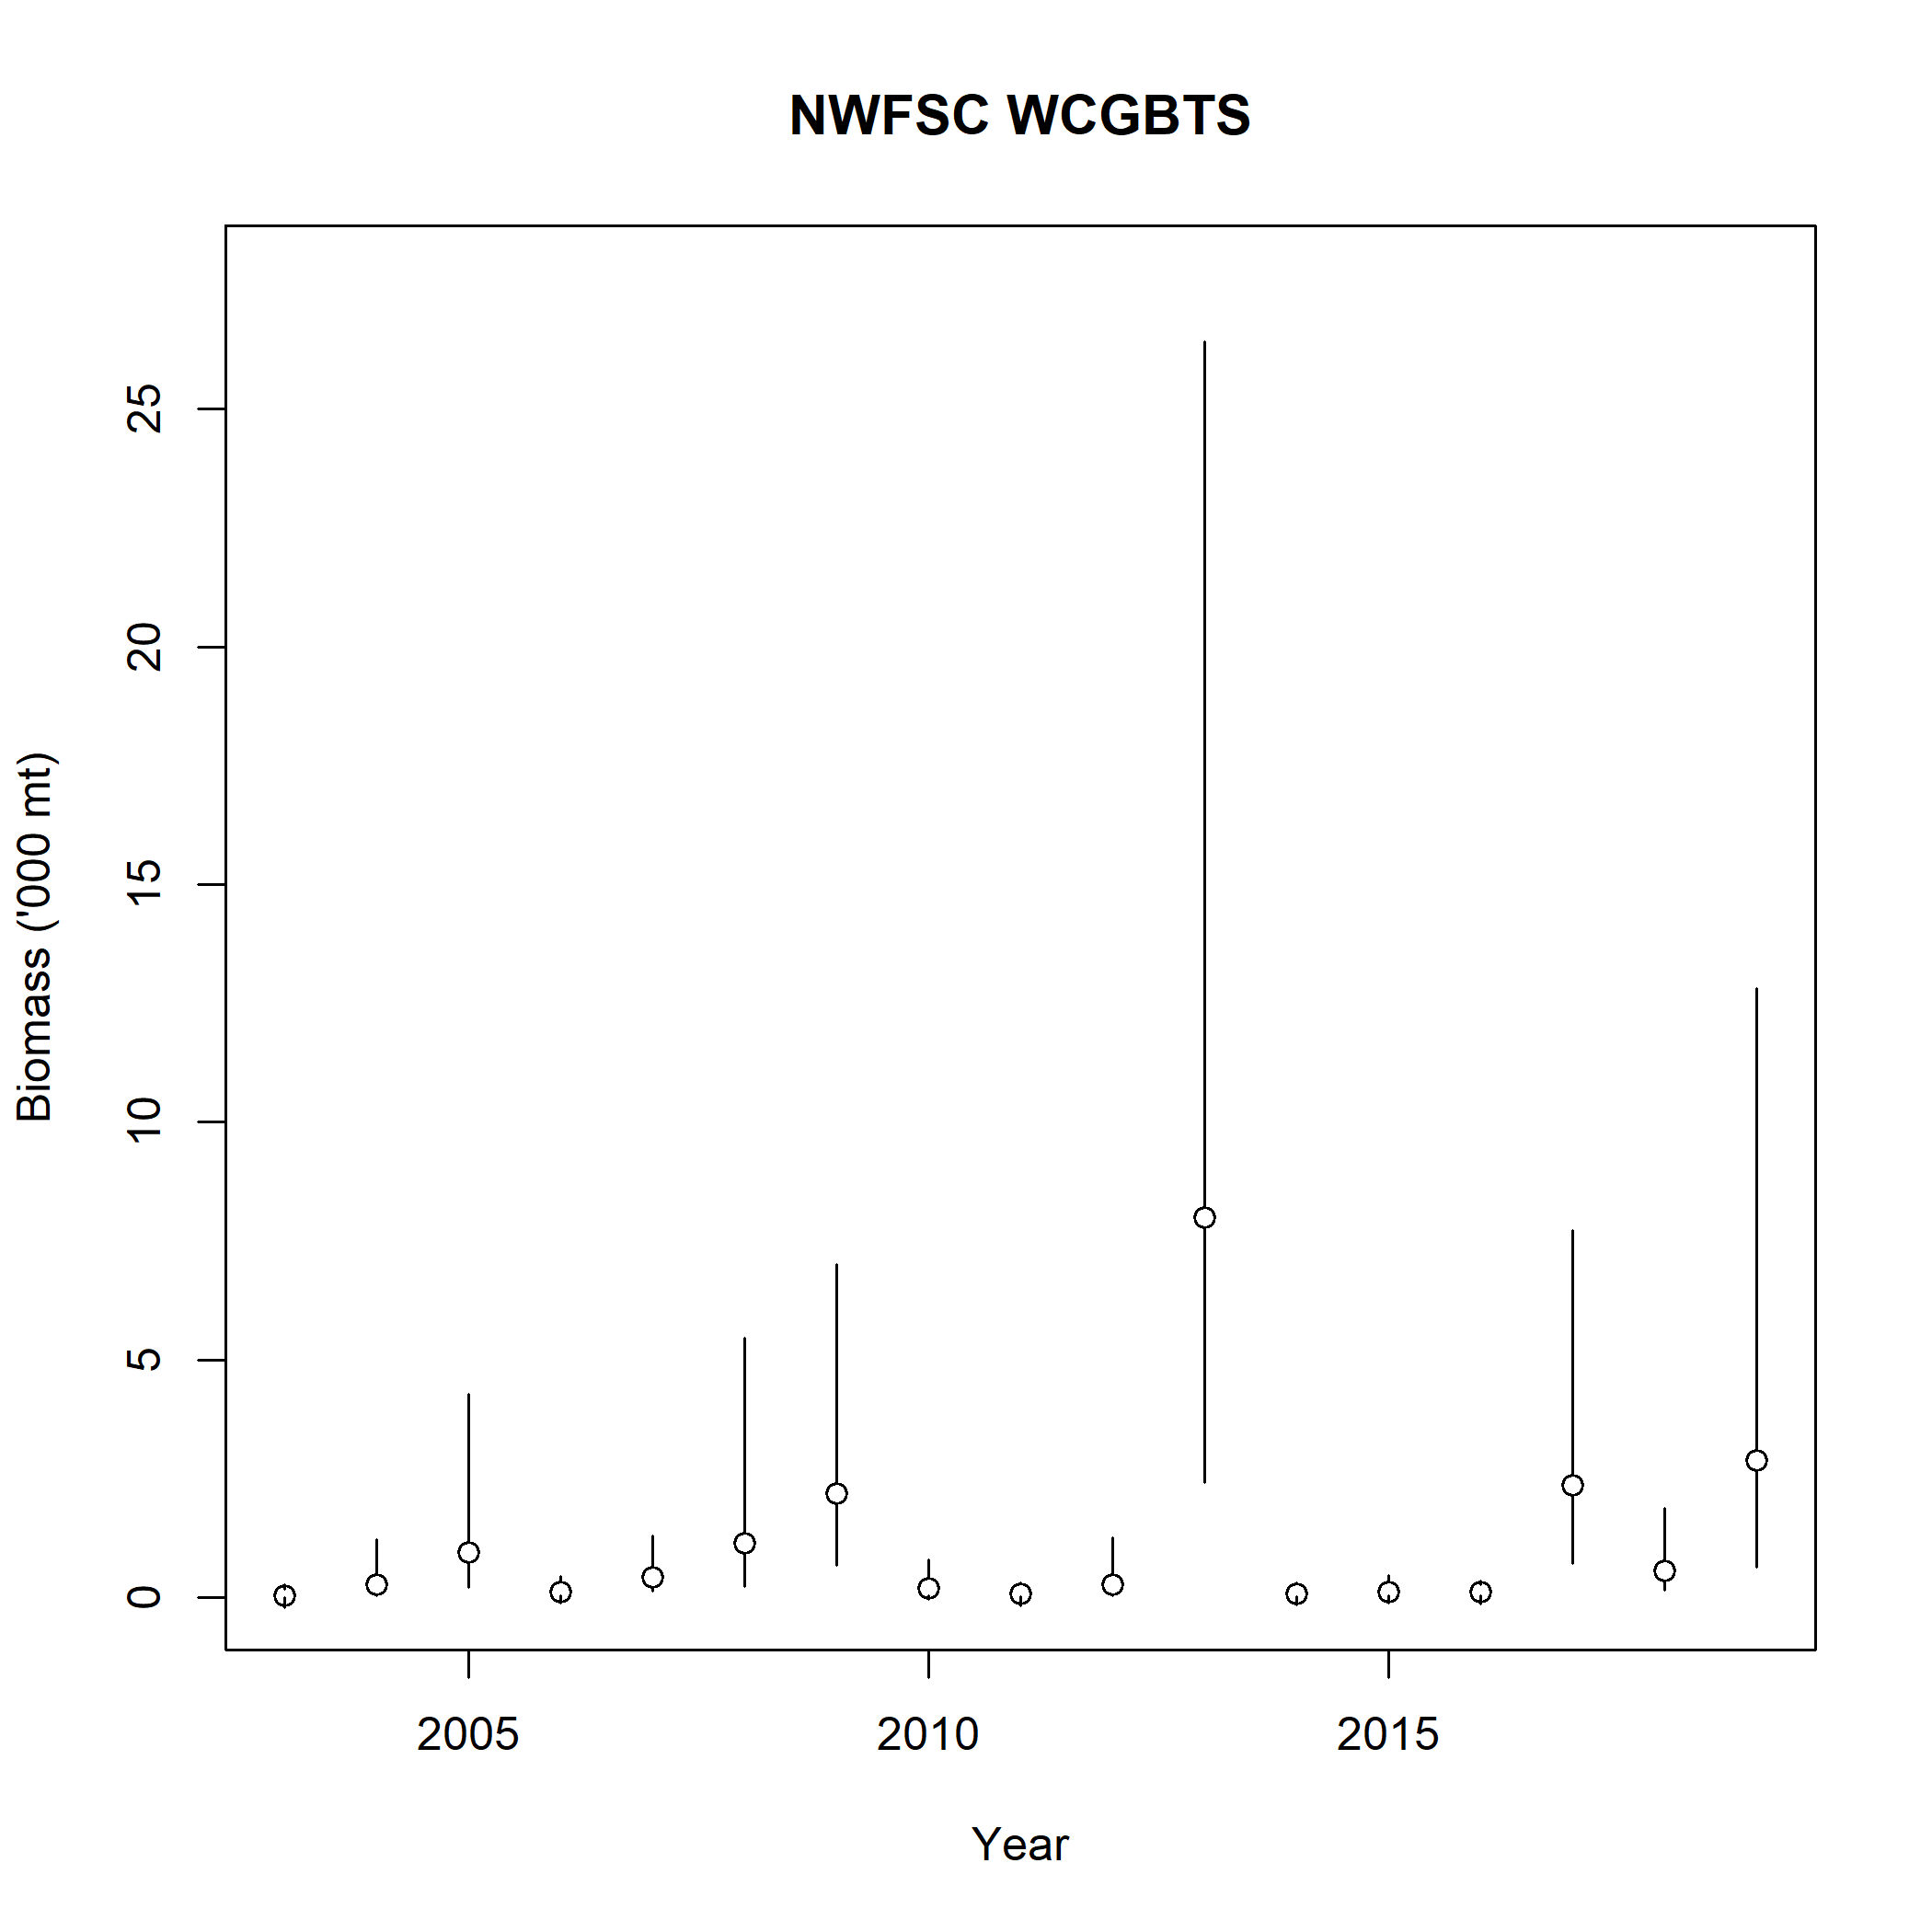
\includegraphics[width=1\textwidth,height=1\textheight]{//nwcfile/FRAM/Assessments/CurrentAssessments/DataModerate_2021/Squarespot_Rockfish/data/Trawl Survey Catch/plots/NWFSC WCGBTS_designed_based_index.png}
\caption{Design-based index of abundance for the NWFSC WCGBT survey.\label{fig:wcgbts-dbindex}}
\end{figure}

\tagmcend\tagstructend

\tagstructbegin{tag=Figure,alttext={Survey length-at-weight data with sex specific estimated fits and comparison to literature lengtha-at-weight values.}}\tagmcbegin{tag=Figure}

\begin{figure}
\centering
\includegraphics[width=1\textwidth,height=1\textheight]{//nwcfile/FRAM/Assessments/CurrentAssessments/DataModerate_2021/Squarespot_Rockfish/data/biology/plots/Length_Weight_All_w_Love_Ests.png}
\caption{Survey length-at-weight data with sex specific estimated fits and comparison to literature lengtha-at-weight values.\label{fig:len-weight}}
\end{figure}

\tagmcend\tagstructend

\tagstructbegin{tag=Figure,alttext={Observed length-at-age by data source.}}\tagmcbegin{tag=Figure}

\begin{figure}
\centering
\includegraphics[width=1\textwidth,height=1\textheight]{//nwcfile/FRAM/Assessments/CurrentAssessments/DataModerate_2021/Squarespot_Rockfish/data/biology/plots/doc_Data_Length_Age_by_Source.png}
\caption{Observed length-at-age by data source.\label{fig:len-age-data}}
\end{figure}

\tagmcend\tagstructend

\tagstructbegin{tag=Figure,alttext={Length-at-age estimated from the NWFSC WCGBT and Hook and Line survey data with sex specific estimated growth.}}\tagmcbegin{tag=Figure}

\begin{figure}
\centering
\includegraphics[width=1\textwidth,height=1\textheight]{//nwcfile/FRAM/Assessments/CurrentAssessments/DataModerate_2021/Squarespot_Rockfish/data/biology/plots/doc_Length_Age_by_Sex_RE.png}
\caption{Length-at-age estimated from the NWFSC WCGBT and Hook and Line survey data with sex specific estimated growth.\label{fig:len-age}}
\end{figure}

\tagmcend\tagstructend

\tagstructbegin{tag=Figure,alttext={Length at age in the beginning of the year in the ending year of the model.}}\tagmcbegin{tag=Figure}

\begin{figure}
\centering
\includegraphics[width=1\textwidth,height=1\textheight]{//nwcfile/FRAM/Assessments/CurrentAssessments/DataModerate_2021/Squarespot_Rockfish/models/Reference model/plots/bio1_sizeatage.png}
\caption{Length at age in the beginning of the year in the ending year of the model.\label{fig:len-age-ss}}
\end{figure}

\tagmcend\tagstructend

\tagstructbegin{tag=Figure,alttext={Maturity as a function of  length.}}\tagmcbegin{tag=Figure}

\begin{figure}
\centering
\includegraphics[width=1\textwidth,height=1\textheight]{//nwcfile/FRAM/Assessments/CurrentAssessments/DataModerate_2021/Squarespot_Rockfish/models/Reference model/plots/bio6_maturity.png}
\caption{Maturity as a function of length.\label{fig:maturity}}
\end{figure}

\tagmcend\tagstructend

\tagstructbegin{tag=Figure,alttext={Fecundity as a function of length.}}\tagmcbegin{tag=Figure}

\begin{figure}
\centering
\includegraphics[width=1\textwidth,height=1\textheight]{//nwcfile/FRAM/Assessments/CurrentAssessments/DataModerate_2021/Squarespot_Rockfish/models/Reference model/plots/bio9_fecundity_len.png}
\caption{Fecundity as a function of length.\label{fig:fecundity}}
\end{figure}

\tagmcend\tagstructend

\tagstructbegin{tag=Figure,alttext={Selectivity at length by fleet.}}\tagmcbegin{tag=Figure}

\begin{figure}
\centering
\includegraphics[width=1\textwidth,height=1\textheight]{//nwcfile/FRAM/Assessments/CurrentAssessments/DataModerate_2021/Squarespot_Rockfish/models/Reference model/plots/sel01_multiple_fleets_length1.png}
\caption{Selectivity at length by fleet.\label{fig:selex}}
\end{figure}

\tagmcend\tagstructend

\tagstructbegin{tag=Figure,alttext={Pearson residuals for combind recreational and commercial fleet. Closed bubble are positive residuals (observed > expected) and open bubbles are negative residuals (observed < expected).}}\tagmcbegin{tag=Figure}

\begin{figure}
\centering
\includegraphics[width=1\textwidth,height=1\textheight]{//nwcfile/FRAM/Assessments/CurrentAssessments/DataModerate_2021/Squarespot_Rockfish/models/Reference model/plots/comp_lenfit_residsflt1mkt0_page3.png}
\caption{Pearson residuals for combind recreational and commercial fleet. Closed bubble are positive residuals (observed \textgreater{} expected) and open bubbles are negative residuals (observed \textless{} expected).\label{fig:rec-com-pearson}}
\end{figure}

\tagmcend\tagstructend

\tagstructbegin{tag=Figure,alttext={Mean length for combined recreational and commercial lengths with 95 percent confidence intervals based on current samples sizes.}}\tagmcbegin{tag=Figure}

\begin{figure}
\centering
\includegraphics[width=1\textwidth,height=1\textheight]{//nwcfile/FRAM/Assessments/CurrentAssessments/DataModerate_2021/Squarespot_Rockfish/models/Reference model/plots/comp_lenfit_data_weighting_TA1.8_Comm_Rec.png}
\caption{Mean length for combined recreational and commercial lengths with 95 percent confidence intervals based on current samples sizes.\label{fig:rec-com-mean-len-fit}}
\end{figure}

\tagmcend\tagstructend

\tagstructbegin{tag=Figure,alttext={Pearson residuals for NWFSC Hook and Line fleet. Closed bubble are positive residuals (observed > expected) and open bubbles are negative residuals (observed < expected).}}\tagmcbegin{tag=Figure}

\begin{figure}
\centering
\includegraphics[width=1\textwidth,height=1\textheight]{//nwcfile/FRAM/Assessments/CurrentAssessments/DataModerate_2021/Squarespot_Rockfish/models/Reference model/plots/comp_lenfit_residsflt2mkt0.png}
\caption{Pearson residuals for NWFSC Hook and Line fleet. Closed bubble are positive residuals (observed \textgreater{} expected) and open bubbles are negative residuals (observed \textless{} expected).\label{fig:hkl-pearson}}
\end{figure}

\tagmcend\tagstructend

\tagstructbegin{tag=Figure,alttext={Mean length for NWFSC Hook and Line lengths with 95 percent confidence intervals based on current samples sizes.}}\tagmcbegin{tag=Figure}

\begin{figure}
\centering
\includegraphics[width=1\textwidth,height=1\textheight]{//nwcfile/FRAM/Assessments/CurrentAssessments/DataModerate_2021/Squarespot_Rockfish/models/Reference model/plots/comp_lenfit_data_weighting_TA1.8_HKL.png}
\caption{Mean length for NWFSC Hook and Line lengths with 95 percent confidence intervals based on current samples sizes.\label{fig:hkl-mean-len-fit}}
\end{figure}

\tagmcend\tagstructend

\tagstructbegin{tag=Figure,alttext={Fit to the NWFSC Hook and Line index of abundance.}}\tagmcbegin{tag=Figure}

\begin{figure}
\centering
\includegraphics[width=1\textwidth,height=1\textheight]{//nwcfile/FRAM/Assessments/CurrentAssessments/DataModerate_2021/Squarespot_Rockfish/models/Reference model/plots/index2_cpuefit_HKL.png}
\caption{Fit to the NWFSC Hook and Line index of abundance.\label{fig:hkl-index-fit}}
\end{figure}

\tagmcend\tagstructend

\tagstructbegin{tag=Figure,alttext={Aggregated length comps over all years.}}\tagmcbegin{tag=Figure}

\begin{figure}
\centering
\includegraphics[width=1\textwidth,height=1\textheight]{//nwcfile/FRAM/Assessments/CurrentAssessments/DataModerate_2021/Squarespot_Rockfish/models/Reference model/plots/comp_lenfit__aggregated_across_time.png}
\caption{Aggregated length comps over all years.\label{fig:agg-len-fit}}
\end{figure}

\tagmcend\tagstructend

\tagstructbegin{tag=Figure,alttext={Estimated time series of spawning output.}}\tagmcbegin{tag=Figure}

\begin{figure}
\centering
\includegraphics[width=1\textwidth,height=1\textheight]{//nwcfile/FRAM/Assessments/CurrentAssessments/DataModerate_2021/Squarespot_Rockfish/models/Reference model/plots/ts7_Spawning_output_with_95_asymptotic_intervals_intervals.png}
\caption{Estimated time series of spawning output.\label{fig:ssb}}
\end{figure}

\tagmcend\tagstructend

\tagstructbegin{tag=Figure,alttext={Estimated time series of total biomass.}}\tagmcbegin{tag=Figure}

\begin{figure}
\centering
\includegraphics[width=1\textwidth,height=1\textheight]{//nwcfile/FRAM/Assessments/CurrentAssessments/DataModerate_2021/Squarespot_Rockfish/models/Reference model/plots/ts1_Total_biomass_(mt).png}
\caption{Estimated time series of total biomass.\label{fig:tot-bio}}
\end{figure}

\tagmcend\tagstructend

\tagstructbegin{tag=Figure,alttext={Estimated time series of fraction of unfished spawning output.}}\tagmcbegin{tag=Figure}

\begin{figure}
\centering
\includegraphics[width=1\textwidth,height=1\textheight]{//nwcfile/FRAM/Assessments/CurrentAssessments/DataModerate_2021/Squarespot_Rockfish/models/Reference model/plots/ts9_Relative_spawning_output_intervals.png}
\caption{Estimated time series of fraction of unfished spawning output.\label{fig:depl}}
\end{figure}

\tagmcend\tagstructend

\tagstructbegin{tag=Figure,alttext={Estimated time series of age-0 recruits (1000s).}}\tagmcbegin{tag=Figure}

\begin{figure}
\centering
\includegraphics[width=1\textwidth,height=1\textheight]{//nwcfile/FRAM/Assessments/CurrentAssessments/DataModerate_2021/Squarespot_Rockfish/models/Reference model/plots/ts11_Age-0_recruits_(1000s)_with_95_asymptotic_intervals.png}
\caption{Estimated time series of age-0 recruits (1000s).\label{fig:recruits}}
\end{figure}

\tagmcend\tagstructend

\tagstructbegin{tag=Figure,alttext={Stock-recruit curve. Point colors indicate year, with warmer colors indicating earlier years and cooler colors in showing later years.}}\tagmcbegin{tag=Figure}

\begin{figure}
\centering
\includegraphics[width=1\textwidth,height=1\textheight]{//nwcfile/FRAM/Assessments/CurrentAssessments/DataModerate_2021/Squarespot_Rockfish/models/Reference model/plots/SR_curve.png}
\caption{Stock-recruit curve. Point colors indicate year, with warmer colors indicating earlier years and cooler colors in showing later years.\label{fig:bh-curve}}
\end{figure}

\tagmcend\tagstructend

\tagstructbegin{tag=Figure,alttext={Estimated 1 - relative spawning ratio (SPR) by year.}}\tagmcbegin{tag=Figure}

\begin{figure}
\centering
\includegraphics[width=1\textwidth,height=1\textheight]{//nwcfile/FRAM/Assessments/CurrentAssessments/DataModerate_2021/Squarespot_Rockfish/models/Reference model/plots/SPR2_minusSPRseries.png}
\caption{Estimated 1 - relative spawning ratio (SPR) by year.\label{fig:1-spr}}
\end{figure}

\tagmcend\tagstructend

\tagstructbegin{tag=Figure,alttext={Equilibrium yield curve for the base case model. Values are based on the 2020 fishery selectivity and with steepness fixed at 0.72.}}\tagmcbegin{tag=Figure}

\begin{figure}
\centering
\includegraphics[width=1\textwidth,height=1\textheight]{//nwcfile/FRAM/Assessments/CurrentAssessments/DataModerate_2021/Squarespot_Rockfish/models/Reference model/plots/yield2_yield_curve_with_refpoints.png}
\caption{Equilibrium yield curve for the base case model. Values are based on the 2020 fishery selectivity and with steepness fixed at 0.72.\label{fig:yield}}
\end{figure}

\tagmcend\tagstructend

\newpage

\clearpage

\tagstructbegin{tag=H1}\tagmcbegin{tag=H1}

\hypertarget{appendix-a.-detailed-fit-to-length-composition-data}{%
\section{Appendix A. Detailed Fit to Length Composition Data}\label{appendix-a.-detailed-fit-to-length-composition-data}}

\leavevmode\tagmcend\tagstructend

\tagstructbegin{tag=Figure,alttext={Length comps, whole catch, Comm_Rec (plot 1 of 3).<br><br>'N adj.' is the input sample size after data-weighting adjustment. N eff. is the calculated effective sample size used in the McAllister-Iannelli tuning method..}}\tagmcbegin{tag=Figure}

\begin{figure}
\centering
\includegraphics[width=1\textwidth,height=1\textheight]{//nwcfile/FRAM/Assessments/CurrentAssessments/DataModerate_2021/Squarespot_Rockfish/models/Reference model/plots/comp_lenfit_flt1mkt0_page1.png}
\caption{Length comps, whole catch, Comm\_Rec (plot 1 of 3).`N adj.' is the input sample size after data-weighting adjustment. N eff. is the calculated effective sample size used in the McAllister-Iannelli tuning method..\label{fig:comp_lenfit_flt1mkt0_page1}}
\end{figure}

\tagmcend\tagstructend

\tagstructbegin{tag=Figure,alttext={Length comps, whole catch, Comm_Rec (plot 2 of 3).}}\tagmcbegin{tag=Figure}

\begin{figure}
\centering
\includegraphics[width=1\textwidth,height=1\textheight]{//nwcfile/FRAM/Assessments/CurrentAssessments/DataModerate_2021/Squarespot_Rockfish/models/Reference model/plots/comp_lenfit_flt1mkt0_page2.png}
\caption{Length comps, whole catch, Comm\_Rec (plot 2 of 3).\label{fig:comp_lenfit_flt1mkt0_page2}}
\end{figure}

\tagmcend\tagstructend

\tagstructbegin{tag=Figure,alttext={Length comps, whole catch, Comm_Rec (plot 3 of 3).}}\tagmcbegin{tag=Figure}

\begin{figure}
\centering
\includegraphics[width=1\textwidth,height=1\textheight]{//nwcfile/FRAM/Assessments/CurrentAssessments/DataModerate_2021/Squarespot_Rockfish/models/Reference model/plots/comp_lenfit_flt1mkt0_page3.png}
\caption{Length comps, whole catch, Comm\_Rec (plot 3 of 3).\label{fig:comp_lenfit_flt1mkt0_page3}}
\end{figure}

\tagmcend\tagstructend

\tagstructbegin{tag=Figure,alttext={Length comps, whole catch, HKL.<br><br>'N adj.' is the input sample size after data-weighting adjustment. N eff. is the calculated effective sample size used in the McAllister-Iannelli tuning method..}}\tagmcbegin{tag=Figure}

\begin{figure}
\centering
\includegraphics[width=1\textwidth,height=1\textheight]{//nwcfile/FRAM/Assessments/CurrentAssessments/DataModerate_2021/Squarespot_Rockfish/models/Reference model/plots/comp_lenfit_flt2mkt0.png}
\caption{Length comps, whole catch, HKL.`N adj.' is the input sample size after data-weighting adjustment. N eff. is the calculated effective sample size used in the McAllister-Iannelli tuning method..\label{fig:comp_lenfit_flt2mkt0}}
\end{figure}

\tagmcend\tagstructend
\end{document}
